\renewcommand\arcmin{\mbox{$^\prime$}}
\renewcommand\arcsec{\mbox{$^{\prime\prime}$}}
% Above taken straight from aastex63.cls, needed for use with other cls files

\newcommand{\rts}[1]{{\color{violet} RTS: #1}} % RTS comment
\newcommand{\jdp}[1]{{\color{red} JDP: #1}} % JDP comment
\newcommand{\cck}[1]{{\color{brown} CCK: #1}} % CCK comment
\newcommand{\amy}[1]{{\color{cyan} ARW: #1}}

% #1- element #2- ionization state #3 -wavelength in angstroms
\newcommand{\spectralline}[3]{#1\,{\textsc{#2}}\ #3\,\AA } % cck fixed up typesetting of this command....
\newcommand{\ov}{\spectralline{O}{v}{629.7}}
\newcommand{\oiii}{\spectralline{O}{iii}{599.6}}
\newcommand{\oiv}{\spectralline{O}{iv}{608.4}}
\newcommand{\mgxbright}{\spectralline{Mg}{x}{609.8}}
\newcommand{\mgxdim}{\spectralline{Mg}{x}{624.9}}
\newcommand{\hei}{\spectralline{He}{i}{584.3}}
\newcommand{\heii}{\spectralline{He}{ii}{304}}
\newcommand{\siiv}{\spectralline{Si}{iv}{1394}}

%ESIS pointing info
\newcommand{\esispointing}{[18\arcsec, -19\arcsec]}
\newcommand{\esisroll}{$.85^{\circ}$}
\newcommand{\esisfov}{11.5\arcmin}
\newcommand{\aianearapogee}{\jdp{update this}\,UTC}





% This gives us \sout for striking out text in comments....
% \sout command defined in aastex63.cls

\title{First Flight of the EUV Snapshot Imaging Spectrograph (ESIS)}

\author{Jacob D. Parker}
\author{Roy Smart}
\author{Charles Kankelborg}
\author{Amy Winebarger}
\author{Nelson Goldsworth}

\begin{abstract}
    The Extreme-ultraviolet Snapshot Imaging Spectrograph (ESIS) was launched on a sounding rocket from White Sands Missile Range on September 30, 2019.
    ESIS is a Computed Tomography Imaging Spectrograph (CTIS) designed to capture both spectral and spatial information simultaneously over a large field of view to provide velocity information on small scale transient events that are prevalent at transition region temperatures.
    In this paper, we review the ESIS instrument, mission, and the data captured.
    We demonstrate how this unique data set can be interpreted qualitatively, and further present some initial quantitative inversions of the data.
    Using a Multiplicative Algebraic Reconstruction Technique (MART) we are able to combine information from all four ESIS channels into a single spatial-spectral cube at every exposure.
    We analyze two small explosive events in the \ov \ spectral line with jets  near $\pm 100$\,km/s that evolve on 10\,s time scales and vary significantly over small spatial scales.
    In the 5 minutes of observing time, ESIS captured tens of the small events across the $\approx 11'$ field of view, as well as several larger extended eruptions, demonstrating the advantage of CTIS instruments over traditional slit spectrographs in capturing the spatial and spectral information of dynamic solar features across large fields of view.
  	
\end{abstract} 

\section{Introduction}

    Observationally, the solar transition region (TR) refers to the portion of the solar atmosphere at temperatures between 20,000\,K and 800,000\,K. 
    Initially, the transition region was viewed as simply the thin interface region between the dense, cool chromosphere and tenuous, million-degree corona, where the temperature of the plasma dramatically increased two orders of magnitude over tens of kilometers \citep[see][and references therein]{tian2017}. 
    Though undoubtedly this type of transition region exists in hot coronal loops, the concept of the transition region has been expanded over the last twenty years to include a dynamic and complicated three-dimensional geometry. 
    It is in the low transition region where the magnetic pressure begins dominate the plasma pressure. \amy{incomplete thought?} The transition region is rife with magnetically driven phenomena such as explosive events \cite[e.g.,][]{dere1991} and microflares \citep{gontikakis2012} and associated flows of 100+\,km/s.
    
    Explosive events have been found to present in different ways and have been observed by many instruments since their original discovery.
    \citet{innes1997} found fast bi-directional jets in \siiv \ line profiles taken by the  SUMER \amy{spell out acronym} \citep{SUMER} separated by a few arcseconds and inferred they must be associated with the outflows of an inclined reconnection current sheet.
    Higher resolution observations from the Interface Region Imaging Spectrograph \citep[IRIS]{depontieu2014} have shown that Si\,{\sc iv} line profiles often show very bright line cores with broad wings and very non-gaussian, more triangular presentations. \amy{add ref?}
    This enhanced line core emission points to a larger amount of stationary plasma, and has been attributed to the presence of a dominate Tearing Mode Instability during the reconnection \citep{Innes2015}.
    Enhanced emission in the line core of a larger explosive event viewed in \heii \ by MOSES \amy{acronyn} has also been attributed to the tearing mode instability \citep{Fox10} despite tens of smaller events in the same data having clear bi-modal profiles \citep{Rust2019}.
    In order to determine which, if any, of these presentations is \amy{missing word} we require high cadence velocity data over a wide range of temperatures simultaneously, something difficult to achieve even in multi-instrument studies.
    
    
    Investigations of TR events to date are severely limited by available observational capabilities. 
    Historically, slit spectrographs have been used to  study\amy{insted of study, "determine velocity of the plasma  in"?} the solar atmosphere.   
    Two-dimensional spectral information must be built by rastering the slit over the region of interest, which takes much longer than the timescales of TR phenomena and confuses whether events are evolving temporally or varying spatially.  
    
    One solution to simultaneously capture spatial and spectral information over a large field of view is to use a slitless imaging spectrograph.  
    The data from these instruments, sometimes called overlapograms, have spatial and spectral information overlapped in the dispersive direction, requiring the data to be inverted or unfolded.
    The difficulty in unfolding slitless spectrograph data has limited its usefulness for extended astrophysical objects like the Sun. 
    Only two satellite missions have routinely captured solar slitless spectrograph data; {\it Skylab} \citep{Tousey1973} and the Res-K instrument of the Russian KRONOS-I mission \citep{Zhitnik1998}, though others have been recently developed and proposed \citep{winebarger2019,golub2020}. 
    Additionally, the currently-operating Extreme-ultraviolet Imaging Spectrograph (EIS; \citet{culhane2007}) on the {\it Hinode} mission \citep{kosugi2007} includes 40\arcsec\ and 266\arcsec\ slots that can produce overlappogram data.  
    Though EIS slot data are not often taken for scientific analysis, they have been used as a flare trigger and since analyzed to aid in interpretation of impulsive phase of solar flares \citep{harra2017,harra2020}.
    In addition to these satellite observatories, there have been several solar observations with slitless spectrographs on sounding rocket flights, including the Multi-Order Solar EUV Spectrograph (MOSES) instrument by Kankelborg and collaborators \citep{Kankelborg01,Fox10}.
    MOSES captured the zero and plus and minus one order of the \heii \ line simultaneously. 
    Doppler shifts were then detected as the spectral displacements in opposite directions in the $\pm$ 1 orders.
    
    Slitless spectrograph data can be thought of as a projection of a three dimensional spatial-spectral data cube, $I(x,y,\lambda)$, onto a two dimensional detector.  
    Although Skylab had just a single projection through $x,y,\lambda$-space, it was possible under some circumstances to determine line intensities and line ratios \cite[e.g.,][]{Keenan1988, Tayal1989, Keenan2006}, and even Doppler shifts \citep{MariskaDoppler1992}. 
%    \jdp{Maybe in O V even!} Nope, Ne VII
    Slitless spectrographs using two projections (usually one dispersed, and one undispersed) have proven sufficient to implement an efficient ground-based magnetograph \citep{DeforestStereoscopy2004}, map Doppler shifts in the solar transition region \citep{Courrier2018}, and invert temperature or density information \citep{winebarger2019}. 
    However, as with any tomographic inversion problem \citep{KakSlaney2001}, the fidelity of reconstruction improves dramatically as projections are added. 
    This is particularly true as the complexity of the object increases, causing the overlap of multiple features along the projection. 
    An instrument that captures multiple projections of the spatial-spectral data cube is called a Computed Tomography Imaging Spectrograph  \cite[CTIS,][]{DescourDereniakCTIS1995}.  
    MOSES is an example of a CTIS, as it captured three projections in the $\pm$ 1 and 0 orders.  
    \cite{Fox10} was able to extract line widths and doppler shifts from a relatively complex explosive event observed by MOSES in \heii.  
    \cite{Rust2019} found unambiguous evidence of explosive events with well resolved, double-peaked spectral line profiles in the same data set.
    
    In 2013, the Extreme-ultraviolet Snapshot Imaging Spectrograph (ESIS) was proposed to the NASA Low Cost Access to Space (LCAS) program and subsequently selected.  
    ESIS is a CTIS with four unique projections of the spatial-spectral data cube and is designed to capture velocity information in small-scale reconnection events in the \ov \ emission line that is formed in the solar transition region.  
%    ESIS was designed to be flown on the opposite side of the MOSES optics bench with the intention of both instruments gathering data simultaneously.   
    The ESIS mission was launched from White Sands Missile Range on September 30,  2019; this paper is a description of the ESIS mission, data and preliminary results.  
 %   Unfortunately MOSES was  not operational during the flight  and will not be discussed further.  
    The ESIS experiment, target, and flight is described in Section 2.  
    Section 3 provides information on the data processing.  Preliminary results are given in Section 4; these include both qualitative and quantitative measures of small-scale velocity events in the solar transition region.  The ESIS mission was successful in  observing tens of small-scale reconnection events over the short rocket flight, as well as demonstrating the usefulness of CTIS observations and developing the analysis techniques required to interpret this unique data.


\section{ESIS Mission}

In this section we provide an overview of the ESIS experiment as well as the time and conditions of the ESIS rocket launch and subsequent data collection.   

	\subsection{The Experiment}
	  	
    	The full ESIS experiment includes an optical instrument, a set of detectors, an on board data acquisition system, and ground support equipment and is described in great detail in the preceding paper \citep{ESIS}.
    	The ESIS optical design consists of a single parabolic primary mirror, an octagonal field stop placed at an intermediate focal plane, and 4 spherical diffraction gratings each with their own corresponding CCD detector.
    	Incoming light is focused by the primary mirror onto the octagonal field stop. 
    	The octagonal field stop is $\approx$ 5 mm wide, which is equivalent to roughly 11\arcmin \  when projected onto the sky. 
    	The light that exits the field stop is reimaged  by the four spherical diffraction gratings onto their own CCD.
    % 	operated in frame-transfer mode. Details like this are in the instrument paper 
    	The portion of the solar spectrum that is captured by each detector ranges from $\approx$ 584\,\AA \ to 630\,\AA. 
    	Within this passband the dominant spectral lines are \hei, \oiii, \oiv, \mgxbright, \mgxdim, and \ov.
    	Assuming a log electron density of \SI[per-mode=symbol]{10}{\elementarycharge\per\cm^3} and a quiet sun DEM, combined with the Schmeltz 2012 abundance file \citep{schmelz2012}, Chianti \citep{ChiantiI,ChiantiX} predicts an intensity relative to \ov \ of .7, .13, .06, .37, .12, and 1 respectively.
    	The .37 relative intensity of the \mgxbright \ line includes a contribution from another O\,\textsc{iv} line within .04 angstroms.
    	
    	\amy{suggest adding 0 in front of decimal places.  I think you need to do a little more explanation here - couple more sentences.}
    
 
    	
        \begin{figure}[ht]
			\begin{center}
				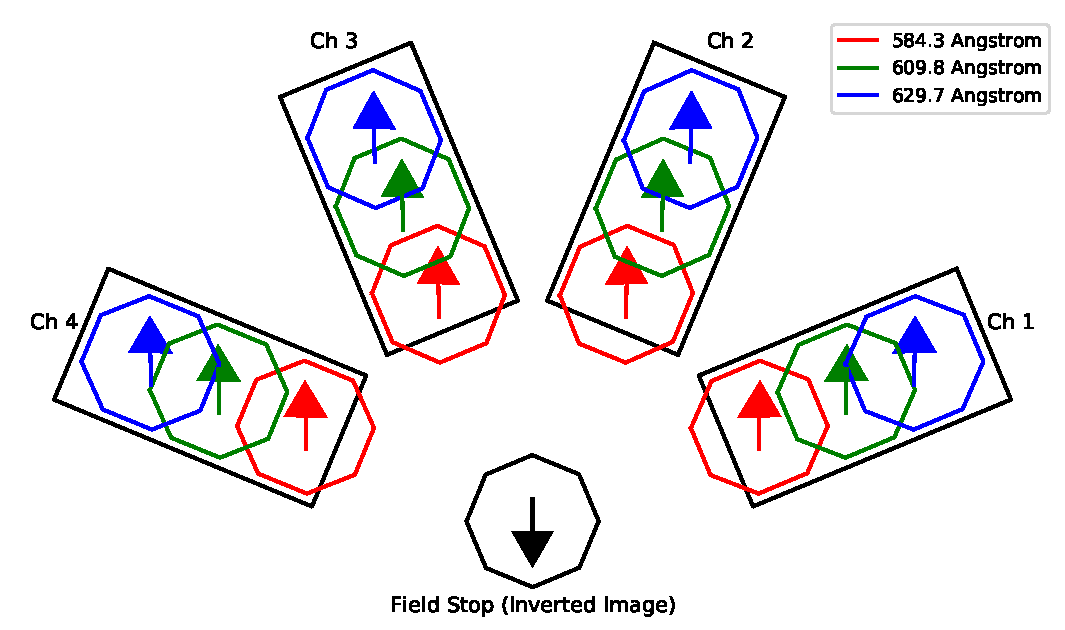
\includegraphics{detector_layout}
				\caption{A modeled layout showing the orientation of each ESIS channels' detector relative to the solar image at the octagonal fieldstop.  The locations of the brightest wavelengths (\hei, \mgxbright, and \ov) in the passband are shown on each detector.  The \hei \ line is designed to hang off the detectors edge, as can be seen in Figure \ref{fig:L0_to_L1}. }
				\label{fig:level_1_array}
			\end{center}
		\end{figure}

\amy{Is that really the orientation of the channels?}
    	
    	
    	Each grating and detector pair, referred in this paper as a channel, is itself an imaging spectrograph.  
    	The channels are arrayed at $45^{\circ}$ increments about the axis of symmetry of the paraboloidal primary mirror such that each channel disperses the solar image a different direction. 
    	Hence, each of these channels capture a unique projection of the spatial spectral cube, shown in Figure \ref{fig:level_1_array}. 
    	As shown, each channel captures the Sun imaged through the octagon and dispersed at different relative angles with respect to solar north. Combining these four channels creates a CTIS. 
    	Exposures from all four channels are gathered nearly simultaneously by triggering the frame transfer in three of the cameras by a single ``master'' camera. 
    	The ESIS instrument currently has 4 channels, but is built to accommodate up to 6 (limited by interference with the optical bench).

    	
        % The dark current in the ESIS cameras is reduced by cooling detectors to low temperatures. 
        % The CCDs in the ESIS cameras are mounted in a copper carrier, which is connected via a copper strap to a cold block.  
        % The cold block is cooled prior during testing and prior to flight to -120 $^{\circ}$C.  This cold block acts as a thermal reservoir to maintain the CCD temperature during the $\sim$ 10 minute rocket flight.   
        % ESIS exposures are transferred via spacewire to an on-board data acquisition system. During ground testing, including alignment, cameras can be commanded individually or collectively and images displayed via ethernet connection to an Operational Ground Support Equipment (GSE) computer.  
        % During flight, ESIS is designed to operate autonomously, though commands can be uplinked if required.  
        % Exposures are buffered, downlinked, and displayed in near real time on the Operational GSE.   These images can be used to make pointing corrections during flight if needed. \amy{This may be too much information, but I wanted to beef up this section.  
        % Also, wanted to highlight  that ESIS isn't just an optical system, it is optical + on board electronics + ground support equipment.}
	
    
	\subsection{Launch and Data Collection} 
		\begin{figure}[ht]
			\begin{center}
				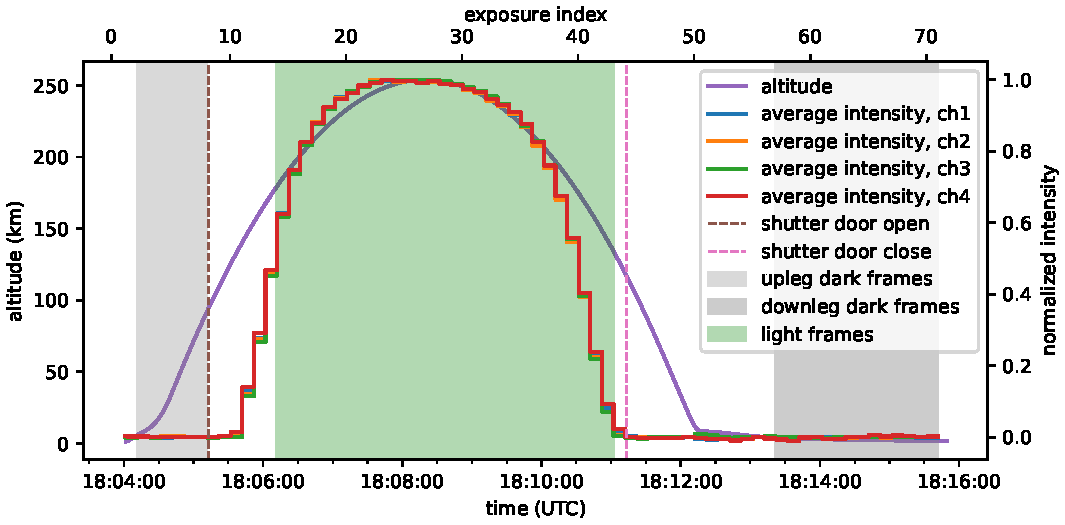
\includegraphics{figures/signal_and_altitude_vs_time}
				\caption{The altitude of the ESIS rocket determined from White Sands Missile Range radar data as a function of elapsed time from launch.  The event times listed in Table~\ref{tab:data_info} are labeled.}
				\label{fig:timeline}
			\end{center}
		\end{figure}

		ESIS was launched at \timeMissionStart~UTC
		on \dateMission\ from White Sands Missile Range.  Figure~\ref{fig:timeline} provides the height of the sounding rocket as a function of time, determined from White Sands Missile Range radar measurements, as well as several key events during the flight.  
		The ESIS cameras began exposing at launch and continued to record full detector ($\sim$2k$\times$1k) images with a 10\,s exposure and cadence throughout the flight. During the initial acceleration phase of the rocket flight, while the shutter door was still closed, these exposures serve as darks.  
		At \timeMissionShutterOpen\ after launch, the shutter door to the experiment opened.  
		The Sun was acquired by the Solar Pointing and Aerobee Control System (SPARCS) and the ring laser gyro (RLG) was enabled at \timeMissionRlgEnable\ indicating the rocket was in Fine Pointing Mode.  
		During this mode, SPARCS maintained a constant target; however, thermal expansion of optical components inside the instrument caused the apparent drift of the solar image on the detectors, as discussed in detail in Section 3.  
		At  \timeMissionShutterClose, the shutter door closed ending solar observations. Exposures continued until the system shutdown at \timeDataStop, providing several additional dark frames at the end of the flight.   A summary of the flight and data collected is given in Table~\ref{tab:data_info}.
		
	    \dateMission\ was a very quiet day on the Sun.  
	    In fact, the last  B-class event detected by GOES \citep{GOES} prior to the ESIS launch was July 7, 2019.  Because of this exceptionally quiet period on the Sun, we chose to point at disk center. 
	    The actual pointing of the center of the ESIS octagonal field stop and roll were found after flight by comparing the ESIS exposure nearest apogee at \timeApogeeFrame\,UTC to the closest AIA\,304\,\AA\ image taken at \aianearapogee.  
	    The ESIS field of view projected onto the AIA 304\,\AA\ image is shown in Figure \ref{fig:fov} as a green octagon.  
	    The pointing was found to be $\approx$ \esispointing \ and the roll offset was found to be $\approx$\esisroll \ (clockwise about Sun center), both within the tolerances for SPARCS pointing.  
	    Figure \ref{fig:fov} shows the full-disk AIA\,304\,\AA\ image. 
	    The ESIS FOV is indicated by the octagon.  
	    
		Each of the ESIS cameras collected 71 images during flight.  The first two images are unusable; the first image has an exposure time of 0\,s and is basically a dump of the dark current in the camera, while the second image has an exposure time slightly longer than 10\,s caused by the cameras syncing to a single trigger of the master camera.  
		All the other images have a 10\,s exposure time.  \amy{double check 30} Thirty of these images were light frames, meaning the shutter door was open and the RLG was enabled. 
		The time during the rocket flight when light frames were collected is shaded green in Figure \ref{fig:timeline}.  
		Light emitted by the Sun is absorbed by the Earth's atmosphere.  
		The degree of absorption depends both on the depth of the atmosphere that the telescope is looking through (i.e., altitude of the rocket) and the wavelength of light.  
		Figure~\ref{fig:timeline} shows the mean intensity in each of the ESIS channels as a function of time.  Atmospheric absorption clearly impacted the observations in the up and down leg of the flight.  
		Accounting for atmospheric absorption will be discussed in Section 3.  
		Though there are \numDataFrames\ light frames, the first and last several frames were greatly impacted by atmospheric absorption and have limited usefulness.  As the rocket was re-entering the atmosphere, there was  ``atmospheric splashdown'' that caused contamination on some of the images that would otherwise be considered darks.  
		This effect can be seen as the small bump in the mean intensities at roughly 18:12:20 in Figure~\ref{fig:timeline}.  
		We restrict the dark frames to the data taken after the first two images, but before the shutter door opened in the upleg, and after atmospheric splashdown in the downleg; these times are shaded with gray in Figure~\ref{fig:timeline}.  
		In total there were \numDarkFrames\ usable dark images.  
		
		
		
		\begin{figure}[ht]
			\begin{center}
				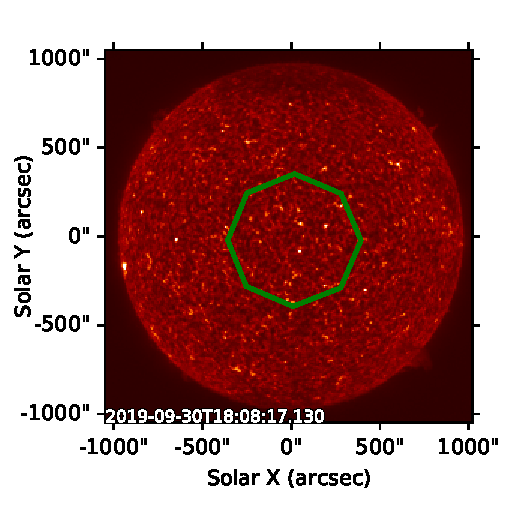
\includegraphics{esis_pointing}
				\caption{\jdp{made smaller for two column, could be changed back easily}The reference AIA 304\,\AA\ data taken at \aianearapogee was used for determining the absolute pointing. The octagon indicates the ESIS FOV.}
				\label{fig:fov}
			\end{center}
		\end{figure}
	

		\begin{table}
		\begin{center}
			\caption{ESIS Flight Data Summary}
			\label{tab:data_info}
			\begin{tabular}{ll|ll}\hline
				Launch Date & \dateMission & Image Size  & \imageShape~pix\\
				Data Acquisition Time & \timeDataStart--\timeDataStop~UTC & Avg. Noise: & \readoutNoise\tablenotemark{a}\\ 
			    Pointing   &  $\approx$ \esispointing & Avg. Gain &   \gain \\
				Field of View  & $\approx$ \esisfov octagonal  & Exposure Time & 10\,s \\
				Roll & $\approx$ \esisroll CW & No. Light Exp: &\numDataFrames\\
			    Spatial  Plate Scale  &  \plateScale & No. Dark Exp: &\numDarkFrames \\
				Spectral  Plate Scale  &  \dispersion & \\
					\hline
			\end{tabular}
		\tablenotetext{a}{Analog-Digital Unit}
		\end{center}
		\end{table}
		
		



	
\section{Data} 

    We have established several levels of data processing that are described in detail below.
    Level-0 represents the raw data that was obtained by the four different cameras during flight.
    Level-1 data prepares raw CCD data for scientific work through a quadrant dependent bias and gain correction, removing non-active pixels, and a dark subtraction.
    Normally, for solar observatories like AIA, higher level data would be further be corrected for solar pointing and roll by interpolating the data into a standard solar map.  
    For ESIS this correction is complicated.  First, the effective pointing of the instrument changed from image to image due to thermal expansion of optical components during the rocket flight.  
    Second the data itself is complicated to represent due to the spatial-spectral overlap on the detector.  
    Third, to retain the most information in the data, it is ideal to include a detailed mapping from the solar spectral cube to each unique detector instead of shifting, rotating, or cropping the detector data.  
    Finally, the ESIS optical instrument distorted the solar image by design. 
    This distortion can be measured and corrected manually, at least for the \ov \ data, by comparing the ESIS data to co-temporal AIA 304\,\AA\ data.  
    To account for  distortion for the full wavelength range requires an accurate optical model.
    Hence, we define two additional levels of data sets.  
    Level-2 data will include updated header information with accurate coefficients of a non-linear and wavelength dependent coordinate mapping from solar coordinates to each detector for each image.   
    It will also be corrected for atmospheric absorption and contain a header keyword tracking the correction as a function of time for use in instrument noise models.
    In addition, Level-2 data will be despiked, and store a mask for future respiking.
    Level-2 data is a necessary step toward fully inverted data products,  but will not be further described here because the results are optical model dependent and currently in development.   
    Instead it will be presented in a forthcoming paper.  
    % Level-2 data will be released at the publication of that paper.  

    In the absence of a complete Level-2 product we seek a shortcut to interpretation of the ESIS data, which allows for taking differences between images and simplified inversions, which we will refer to as Level-3.
    Level-3 data is comprised of a single spectral line cropped from Level 1 data and mapped to the sky plane via a non-linear coordinate transform derived from a coalignment to co-temporal AIA data and an internal coalignment of each ESIS channel to a reference channel.
    
    The highest level data product we envision providing in the future, Level-4, is the spatial-spectral data cube, i.e., the intensity as a function of $[x, y , \lambda]$, which will be the results of various inversion methods.    
    Since inversions generally do not produce unique solutions, there may be multiple Level-4 products obtained by different inversion methods.  
    % Level-4 data products will be described in future publications as they become available.   
    
    Level-1 and Level-3 data will be made publicly available through various solar data archives. Below we describe each completed data set in more detail. 
    
    \subsection{Level-0 Data}
    
        Level-0 data is the raw data collected during the ESIS rocket flight.  
	    Each image was written to a fits files with on-board timestamp, camera number, and other parameters, such as the read out from temperature sensors included in the header.   
	    
	    Each camera includes a detector with 2048 columns and 2064 rows.  The detector is operated in frame transfer mode, meaning the exposed portion of the detector is shifted into a storage portion that is read out during the next exposure. The storage portion is simply a mechanically masked region of the detector. The intention was that the storage region would be 520 rows per quadrant while the exposed region would be 512 rows per quadrant, producing an image that was 1024 rows in total.  An oversight during implementation inverted the size of the storage and exposed region, meaning the final image had 1040 rows.  Having a larger exposed region than storage region implies that eight rows originally exposed at the central portion of the detector were not behind the mechanical mask when the read out was initiated. However, because these rows were only unmasked for roughly 20 ms and the solar flux was low, there was no discernible impact on the data.
	    
	    The data is read out through 4 ports in the detector.  The read out register has 50 additional dummy pixels, or non-active pixels (NAPs), that are read out before each row of the detector data.  When the detector is read out, those 50 pixels are stored as part of the image.  Two additional ``overscan" pixels are read after each row of data and also stored as part of the image.  A stored Level-0 data file, then, is 2152$\times$1040 pixels.   During pre-flight lab testing, it was found that the median intensity in columns 21-50 of the NAPs of each read out port was an excellent proxy for the detector bias.  Additionally the data from each port is converted from analog to digital through a unique circuit.  Though the same components were used, slight variations in the circuits caused slight differences in the gain (elec / DN) and read  noise associated with each quadrant.  The gain for each quadrant in each camera was measured prior to flight.  The noise was measured from usable dark images during flight.  The average and standard deviations in these values are given in Table~\ref{tab:data_info}.
    
    \subsection{Level-1 Data}
	    \begin{figure}
	    	\centering
	    	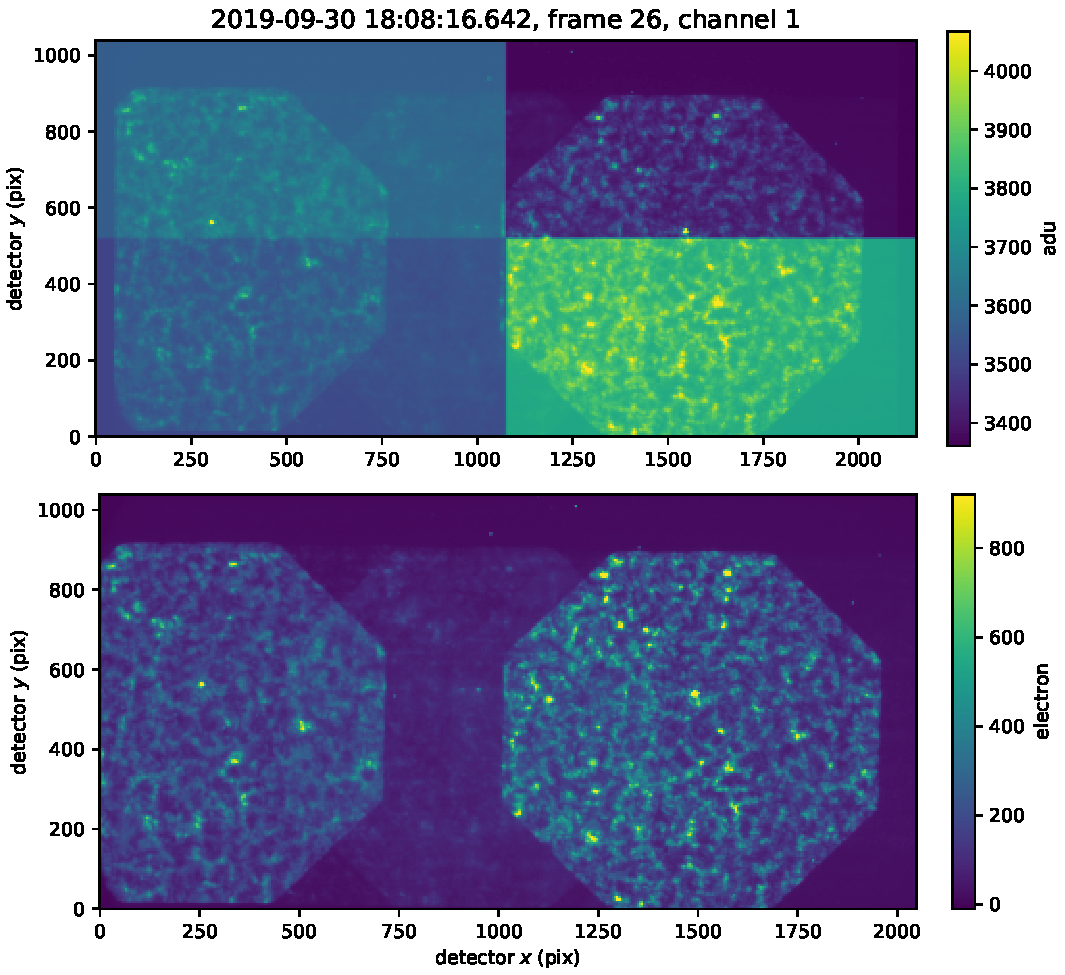
\includegraphics{L0_to_L1}
	    	\caption{The top panel is the raw, Level-0 image captured by Channel \defaultChannel\ of ESIS during apogee. The bottom panel is the same image after Level-1 processing. The Sun viewed through the octagonal field stop in the \ov \ spectral line is on the right side of the detector, this portion of the detector was cropped to generate Level-3 data.  The Sun viewed through the octagonal field stop in the \hei \ line is partially on the left side of the detector. The \mgxbright \ line is between and partially overlapping both of these two strong lines.}
	    	\label{fig:L0_to_L1}
	    \end{figure}
    	
    	A summary of the flight data parameters, as described in the preceding sections, is provided in Table~\ref{tab:data_info}. 
    	For each channel, there were \numDataFrames\ light images that were processed into Level-1 data and \numDarkFrames\ dark images used to process the data.
    	Our procedure to convert from Level-0 to Level-1 is described below. An example of a Level 0 and Level 1 image is shown in Figure~\ref{fig:L0_to_L1}.
    	
    	\begin{enumerate}
    	    \item Calculate and subtract the bias of each quadrant of each usable image (light or dark) by taking the median of columns 21-50 of the NAPs for each read out port.   
    	    \item Create a master dark image for each channel by taking the median along the time axis of all the bias-subtracted usable dark images.
    	    \item Subtract the master dark from each bias-subtracted light image.
    	    \item Crop each image to remove the non-active and overscan pixels.
    	    \item Convert images from DN to electrons by multiplying each quadrant of each image by the gain for that quadrant.
    	\end{enumerate}
    	The resulting Level-1 dataset contains each channel's image sequence in units of photoelectrons.
    	In addition to the images, the Level-1 fits header is updated with the time, exposure length, and altitude associated with each image using standard FITS header keywords.   
	

    \subsection{Level-3 Data} \label{sec:level-3}
 
    
    	\newcommand{\vigfit}{[0.44, 0.34, 0.38, 0.5]}
    	\newcommand{\levthreetime}{2019-09-30T18:08:51.644}
    	
    	The ESIS Level-3 data product is created to provide a co-aligned, single wavelength image in each channel for quick identification of events with significant line-of-sight velocities and easy comparison with coordinated data that does not require inversion. 
    	Level-3 data also allows for single wavelength inversion prior to the completion of the final optical distortion model and the Level-2 data product.  A description of both qualitative and quantitative analysis of Level-3 data is given in Section 4.  Generating Level-3 data products require several steps including 1) converting to  Level-1 data photons and despiking, 2) correcting the optical distortion and internal co-alignment of the four ESIS channels, 3) correcting of each channel for vignetting, including identifying regions where the contributions of the overlapping \mgxbright \ line confuse the \ov \ data, and 4) correcting the relative radiometric differences in each channel.  Each of these corrections are described in detail below. 
    	Figure \ref{fig:coalign}a shows an example of a Level-3 image from Channel 2 \jdp{verify this} taken at \levthreetime.
    	
  		\begin{figure}[htb!]
    		\centering
    		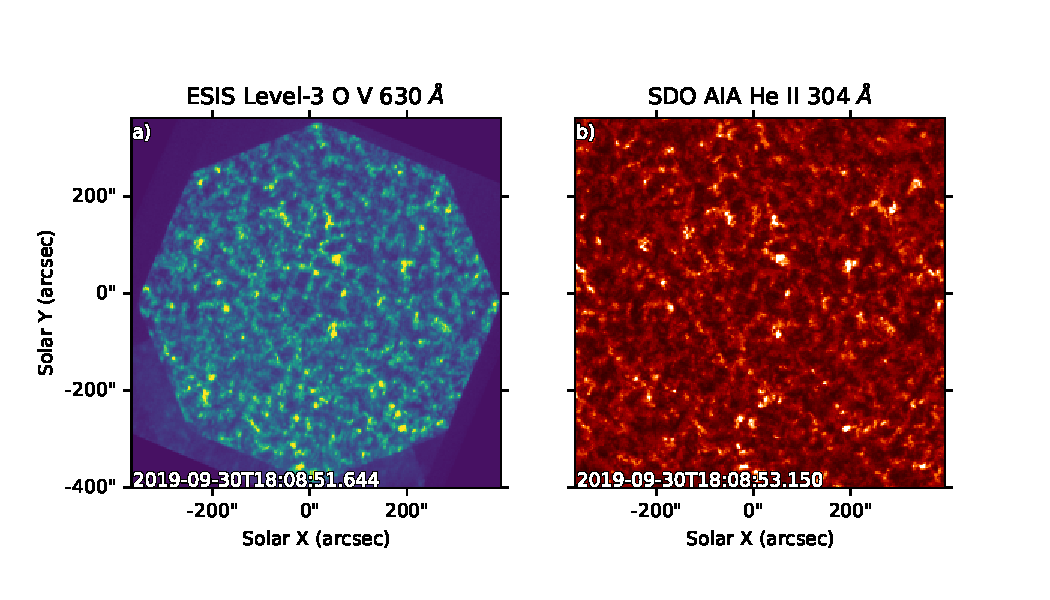
\includegraphics{aia_coalign.pdf}
    		\caption{(a) An example of the Level 3 data product from Channel 1 taken at \levthreetime. This data has been aligned using nonlinear mapping parameters to the closest co-temporal AIA 304\,\AA\ image, shown in (b). }
    		\label{fig:coalign}
    	\end{figure}
    	
    
    \subsubsection{Conversion to Photons and Despiking}
        In order to use Level-3 data for early inversion the intensity needs to  converted to photons in order properly account for uncertainty in the data.
        The conversion from electron to photon is done to Level 1 data prior to co-alignment efforts.
   		The intensity in photons , $I_{\gamma}$, then becomes,
   		\begin{equation}
	   		I_{\gamma} = I_{\SI{}{\elementarycharge}} * 3.6 \frac{\SI{}{\electronvolt}}{\SI{}{\elementarycharge}} * \frac{\lambda}{hc}.
   		\end{equation}
		With a Silicon band gap energy of \SI[per-mode=symbol]{3.6}{\electronvolt\per\elementarycharge}, and an energy per \ov \ photon 
		of \SI[per-mode=symbol]{19.6}{\electronvolt\per\photon}, each count in electrons is $\approxeq .18$\,photons.
		Creating Level-3 data for a different spectral line in the ESIS passband simply requires using a different wavelength when converting to photons.
		
		\amy{suggest giving number in electron / photon.  Add 0 before decimal.}
		
		Due to a substantial number of charged particle hits on the ESIS detectors Level-1 data was also despiked in order to minimize ill effects on co-alignment and inversion.
		\jdp{Taking a stab at this.  Is this right Roy?  Also, do we need this?}
		Our despiking routine is implemented in the following steps:
		\begin{itemize}
		    \item Create one 2-D histogram for each data dimension (image row, image column, and time) comparing each pixel's value to its local median, taken over 11 pixels, for a fixed number of local median bins (128).
		    \item For each local median bin, form a cumilative distribution and identify the intensity value corresponding the to 0th and 99.9th percentile giving two curves (threshold intensity as a function of local median) per histogram.
		    \item Fit a line to each curve with each local median bin weighted by the number of pixels within in each bin.  These lines form the upper and lower intensity thresholds at in each local median bin.
		    \item Replace each pixel that exceeds the upper threshold and falls beneath the lower threshold line (the spikes) with its local mean weighted by kernel k (Equation \ref{eq:despike_kernel}).
		\end{itemize}
	
        The kernel used to determine the replacement value for bad pixels is
		\begin{equation} \label{eq:despike_kernel}
		    k(x) = e^{-|x|/a},
		\end{equation}
	    and is applied in each dimension (image row, image column, and time).
        For our implementation $a=.5$\,pixels and $x= -2, -1, 0, 1 , 2$, the distance in pixels from the value being replaced.  
        
        
    \subsubsection{Optical distortion correction and channel co-alignmentment}
   		
   	    The four ESIS channels were spatially co-aligned in two steps.
        First, each ESIS image is roughly cropped around the \ov \ spectral line, (roughly pixels 1000 - 2048 of the Level-1 data shown in Figure~\ref{fig:L0_to_L1}) and then co-aligned to the closest AIA 304\,\AA\ image in time.  
        The AIA 304 channel was chosen for co-alignment because it is the AIA EUV channel most visually similar to O V, in both the background and bright events (Figure \ref{fig:coalign}b).
        Prior to co-alignment each AIA image was prepped to Level-1.5 using the aiapy routines \texttt{aiapy.calibrate.update\_pointing()} and \texttt{aiapy.calibrate.register()}.
        The co-alignment was achieved through a linear coordinate transformation of the cropped ESIS image that maximizes the zero lag cross-correlation between it and AIA 304, the results of this are shown in Figure \ref{fig:coalign}.
        
    	Since ESIS has a slightly non-linear distortion function \citep{ESIS}, an additional internal alignment step is performed.
    	Using a single ESIS channel as reference, in this case Channel 2, each other channel is co-aligned to it via a quadratic coordinate transformation that maximizes the zero-lag cross-correlation. 
    	Figure \ref{fig:cc} shows the ratio of peak cross-correlation after the quadratic internal alignment to that of the linear co-alignment with AIA for every camera pair and every exposure\amy{; a ratio greater than 1 implies this second step improved co-alignment}.
    	After performing this additional internal alignment we find that not only is the co-alignment between each channel and the reference channel improved (dots in Figure \ref{fig:cc}), but also the co-alignment between every other combination of channels (stars in Figure \ref{fig:cc}).
    	This ratio is greater than 1 in all cases and shows a less than 1 percent improvement in peak correlation, demonstrating the subtle non-linearity of the ESIS optical distortion function.
    	In pixels, this corresponds to an average change in mapping of $\approx$ 0.4 pixels.
    	
        After the co-alignment is complete each Level-3 image has been re-binned to AIA resolution, 0.6 arcsecond per pixel, and can be assigned the WCS information \citep{WCS} from the nearest image AIA in time, providing pointing information and easier co-alignment with coordinating instruments.
    	

    	
     	\begin{figure}[htb!]
    		\centering
    		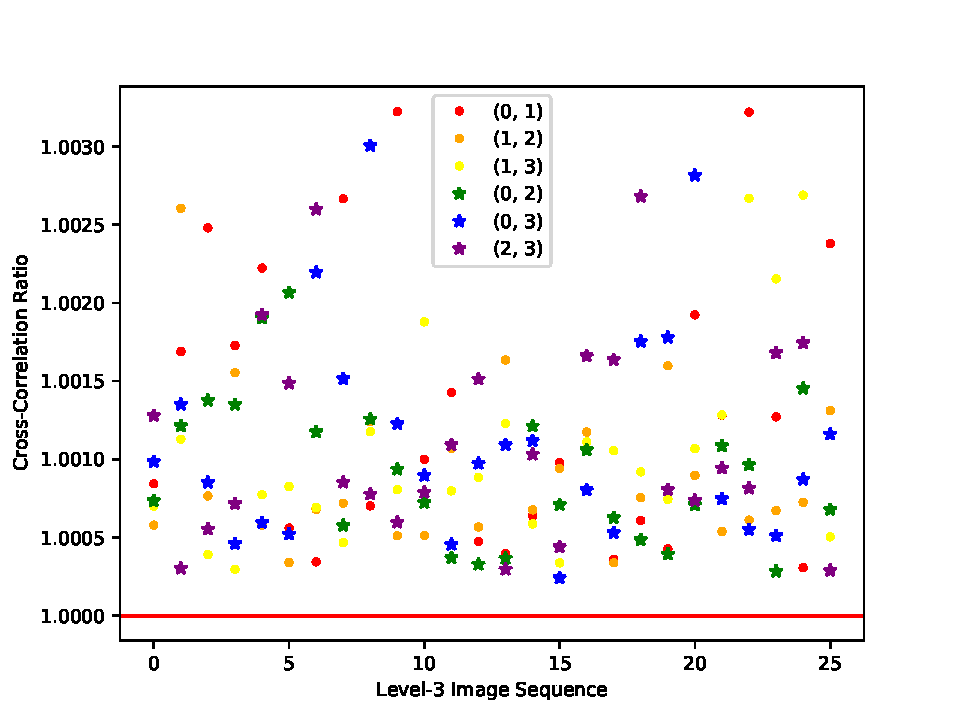
\includegraphics{internal_align.pdf}
    		\caption{\jdp{update channel pairs from (0,1) to (1,2).  1 column width?} For each ESIS exposure (or image sequence) every channel pair, labeled in the legend, is cross-correlated to measure internal alignment quality.  The ratio of zero lag cross-correlation after a quadratic transformation to that of a linear transformation is plotted.  Every point being above the ratio = 1 line indicates improved internal alignment for every combination of ESIS channels at each image sequence.}
    		\label{fig:cc}	
    	\end{figure}
    	
 		\begin{figure}[htb!]
			\centering
			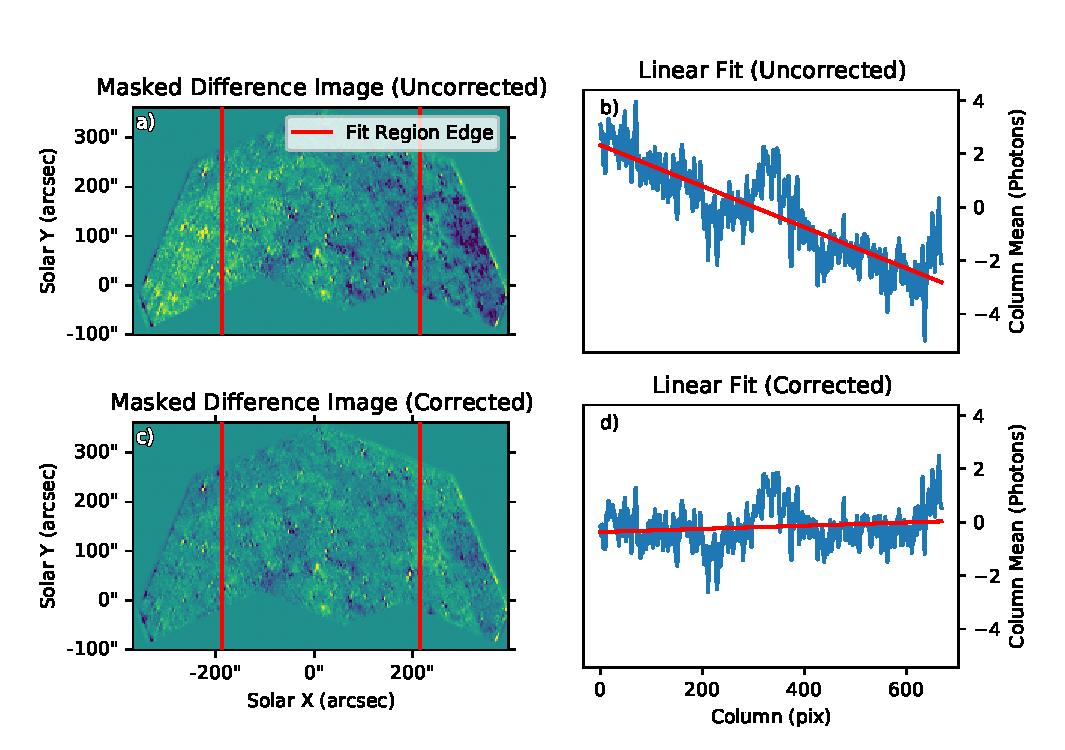
\includegraphics{vig_correct.pdf}
			\caption{\jdp{update}Panels a and c show example difference between images with \mgxbright \ masked that are uncorrected and corrected for vignetting respectively.  The line fit to the column mean as a function of column (fit between the red bars) shows a difference in background of $\approx 5$ photons before correction (panel b) at the edges of the field of view, and .4 photons after (panel d). }
			\label{fig:vig_correct}
		\end{figure}

    \subsubsection{Vignetting correction}
  
        Each ESIS channel has a linear trend in intensity across the octagonal field of view along the dispersion direction due to internal vignetting in the optical system caused by having multiple stops in the optical system \citep{ESIS}.
        In the co-aligned Level-3 images, where solar north is rotated to the top of the image, the dispersion axes runs at different angles relative to solar north in each channel, so the impact of the vignetting field can be seen in the linearly trending background when taking the difference between two channels (Figure \ref{fig:vig_correct}a).
        We seek to minimize the linear trend in intensity seen in Level-3 difference images by dividing out a linearly trending background, aligned to the dispersion axis, in every image.
        
        We define the vignetting field for each channel, $i$ at each time, $s$, as a function of the pixels in the Level-3 data, $(x,y)$, as 
        	\begin{equation}
        		V_{is}(x,y) = \frac{m_i}{r_t} * [r(x,y,s) - r_0] + 1,
        		\label{eqn:vignet}
        	\end{equation}
		where
			\begin{equation}
				r = x_0 + [\cos(\alpha_i)(x-x_0-x_{\text{drift}}*s/s_t) - \sin(\alpha_i)(y-y_0-y_{\text{drift}}*s/s_t)].
				\label{eqn:vignet2}
			\end{equation}
        
        In Equation \ref{eqn:vignet}, $r_0$ is equal to 65 pixels, and represents the distance from the Level-3 image edge to the ESIS field stop octagon edge at $s = 0$, the first Level-3 image.
        The total size of the octagon, $r_t$, is equal to 1140 pixels.
        In Equation \ref{eqn:vignet2},  $\alpha_i$ is the angle of rotation of each ESIS Level-3 image relative to a Level-1 image row.
        In this case, $\alpha_i = [112.5^{\circ}, 67.5^{\circ}, 22.5^{\circ}, -22.5^{\circ}]$ for Channels 1-4, respectively.
        The vignetting field is rotated about the origin of each image in pixels, $[x_0, y_0] = [635,635]$, to account for the change in dispersion direction.
        ESIS images have a slight pointing drift, so the field of view defined by the octagon moves in Level-3 data as a function of time or image sequence, $s$.
        Therefore the vignetting field is translated to follow this drift.
        This is achieved through a change in origin.
        At each time $s$, the origin is translated by $[x_{drift},y_{drift}]*s/s_t = [8_{pix},-4_{pix}]*s/29$, where $s_t $ is the total number, 29, of Level-3 images in time. 
        
        Due to inconsistencies between predicted vignetting field slope and what is seen in the data we choose to fit the linearly trending background in each difference image and use the vignetting field slopes, $m_i$, as free parameters to minimize it.
        We measure the trend in the background by taking the mean of each column in the difference image and fitting a line to it as a function of column position, shown in the right hand column of Figure \ref{fig:vig_correct}.
        The four channels of ESIS give 6 possible difference images for fitting the vignetting function for each image sequence $s$. 
        When the average slope of all 174 fits (6 difference images per each of the \numDataFrames \ exposures) is minimized we consider the vignetting corrected.
        Measuring the trend from the data is additionally complicated by the overlap of the bright \mgxbright \ line.  
        This line overlaps different regions of the field of view in each channel, see Figure~\ref{fig:mgx_overlap}.  
        Therefore when fitting the background we restrict ourselves to the portion of the field of view without the \mgxbright \ overlap in any channel.
        We also only use column means between the red bars in Figure \ref{fig:vig_correct} to ensure sufficient pixel numbers in each column.  
        
        The resulting final fit, $m_i = \vigfit$, gives smaller slopes than are predicted using ray tracing and geometric optical models \citep{ESIS}, which can be attributed to a few likely culprits. 
        One source of error likely comes from the imprint of adjacent spectral lines, the most obvious being that of \mgxdim \ visible in Figure \ref{fig:vig_correct}c.
        Since this Mg {\sc x} line overlaps almost entirely with O {\sc v}, and has an identical vignetting function, it adds intensity that prevents a perfect fit. 
        If this were the only source of discrepancy between the vignetting function predicted by the raytrace and the fits obtained from the data, then we would simply use the same, predicted vignetting for every channel. 
        However, we can anticipate slightly different vignetting in each channel due to variations in assembly so we allow each channels slope to vary independently.
        A misalignment of the ESIS field stop center, the ESIS primary optic center, and the center of the ESIS grating array, all shift the geometry of the ESIS central obscuration and can easily modify the vignetting field in each channel.
        Despite the uncertainties in vignetting, which we have found difficult to quantify, Level-3 differences are much flatter in intensity post vignetting correction as is seen in Figure \ref{fig:vig_correct}c, and will therefore lead to a higher fidelity intensity recovery when inverting Level-3 data.

        
  
        
        \begin{figure}[htb!]
        	\centering
        	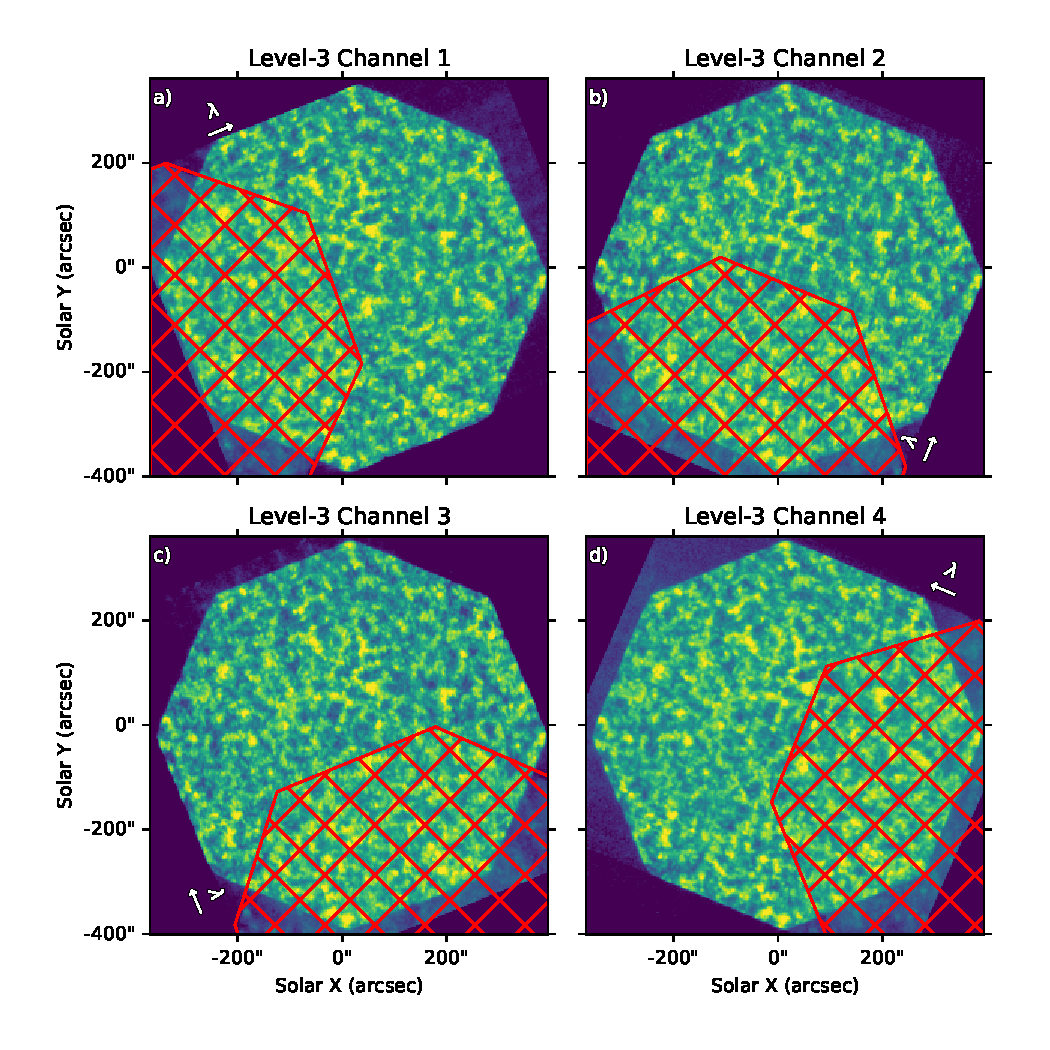
\includegraphics{mgx_overlap.pdf}
        	\caption{\jdp{update}The red hashed region shows the overlap of the \mgxbright \ spectral line in each channel that is masked prior to the vignetting correction and intensity normalization. These images are displayed in log scale in and attempt to bring out the subtle contamination.  The outline of the Mg\,{\sc x} can be seen very clearly in difference images like Figure \ref{fig:l3_dif}. }

        	\label{fig:mgx_overlap}
        \end{figure}
        
        

        
    \subsubsection{Relative Radiometric correction }
        
        Normalizing the intensity of each channel is done by equalizing the image mean over the least contaminated shared piece of sun, and is therefore performed after inter-channel co-alignment and the vignetting correction.
        We divide each image by it's mean in the region of the field of view uncontaminated by \mgxbright \ in everychannel (shape shown in Figure \ref{fig:vig_correct} a and c) and multiplying it by the mean in that same region from the brightest image in the brightest channel (Channel 2 at apogee)
        This not only normalizes the intensity between each channel at every exposure, but also corrects for the effects of atmospheric absorption mentioned in earlier sections. 


\section{Preliminary Results}

	   ESIS is an extremely unique instrument.  It is not only a slitless imaging spectrograph, of which there only a handful of examples, it is also a Computed Tomography Imaging Spectrograph (CTIS).  
	   To our knowledge, the ESIS and MOSES sounding rocket instruments are the only CTIS instruments ever flown to observe the Sun, and  the Advanced Stokes Polarimeter on the Dunn Solar Telescope at the National Solar Observatory is the only ground based CTIS to capture solar data \citep{deforest2004}.  
	   MOSES only took three projections of the spatial-spectral data cube by observing $\pm$ 1 and 0 orders.
	   %, so its data is relatively simple when compared to the ESIS data set.   
	   ESIS added an additional projection, the ability to independently focus each channel, and a explicit field of view defined by the field stop, a significant upgrade in flexibility and data quality over MOSES.
	   In this section, we provide some preliminary analysis of the ESIS Level-3 data to both demonstrate that the ESIS mission accomplished its scientific goal of detecting the velocity signatures of small scale eruptive events, but also to provide useful qualitative and quantitative understanding of this data.  
		
	    Despite the lack of solar activity, ESIS managed to capture tens of small, transient events and one significant eruption during the $\approx$5 minutes of observation in the \ov \ spectral line.  
	    We provide a few examples of these events in this section.  
	   % Additional analysis is provided in a series of upcoming papers.  
	
    \subsection{Level-3 Difference Images} \label{sec:dif_images}
    	Early work with MOSES images demonstrated the utility of examining differences between different projections of the spatial-spectral cube (channels) to identify solar features with significant line-of-sight velocity \citep{Fox10,FoxPhD,RustPhD,Rust2019}, and spectral contamination \citep{RustPhD, Rust2019,Parker2021}.
    	It is for this reason that we developed a spatially co-aligned data product (the Level-3 data) quickly that would allow us to take differences between each ESIS channels.
    	Each ESIS channel disperses solar features in a different direction relative to solar north, determined by the azimuthal position of each grating.
    	The positive dispersion direction in each Level-3 image is indicated by the arrows  in Figure \ref{fig:mgx_overlap}.
    	In the case of an eruptive event with a velocity signature, the Doppler shifted intensity is dispersed a different direction in each channel, meaning taking the difference between two spatially aligned channels leave only intensity away from the spectral line core.  
    	To put it another way, subtracting the data from two channels removes all the spatial structures that overlap in the two channels and leaves only the velocity signatures. 
    	%For our initial analysis, we focus on the dominant O {\sc v} 629.7 \AA \ spectral line in the ESIS passband. \amy{I think this is a given since it is the only one in level3}
    	
    	Figure~\ref{fig:l3_dif} shows the difference between Channels 2 and 3 for the full ESIS field of view.  
    	Several regions of the field of view show black and white features, a few of these are marked with red boxes and will be discussed in detail below.  
    	The small black features tend to lie at an angle -22.5$^\circ$ with solar north, which is the direction of dispersion of Channel 3, while white features tend to lie at an angle of 22.5 $^\circ$ with solar north, which is the direction of dispersion of Channel 2.  
    	Due to the relative orientation of each ESIS channel's dispersion axis, taking the difference of these small events leaves a V-shaped or X-shaped structure in it's place.  
    	Every X or V-shaped features in an ESIS difference image, Figure~\ref{fig:l3_dif}, that have obvious, and nearby, positive and negative portions indicate solar events with significant line-of-sight (LOS) Doppler velocity.   
    	Other things to note in this image is the white octagon that overlays the lower left quadrant of the image, this is the \mgxbright \ line that overlaps the \ov \ line in Channel 2.  The dark octagon on the lower right quadrant is the portion of the \mgxbright \ line that overlaps the \ov \ line in Channel 3.    
   		
   		\begin{figure*}[htb!]
   			\centering
   			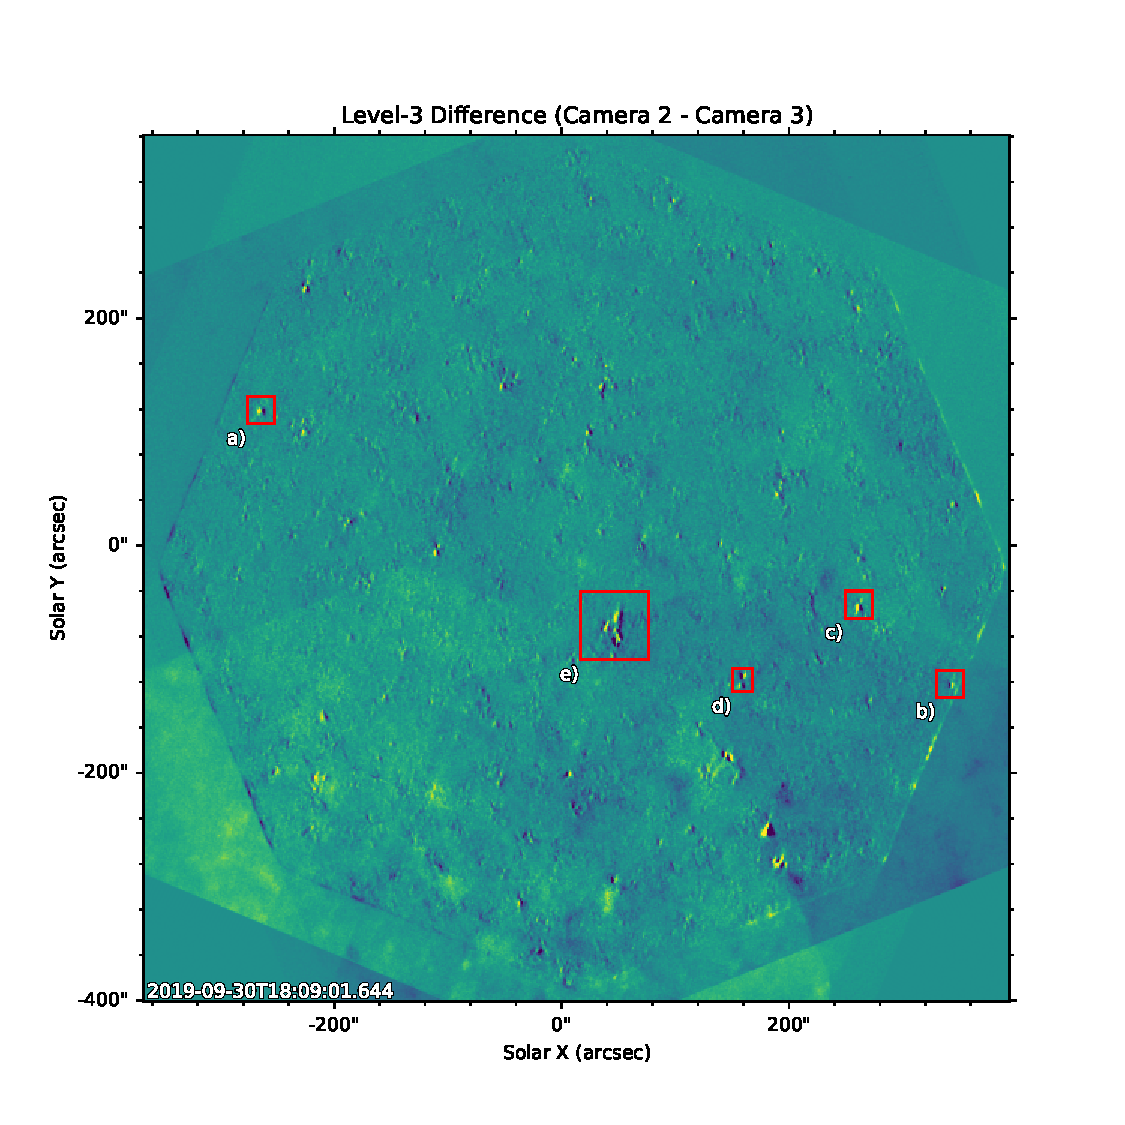
\includegraphics{l3_dif}
   			\caption{Full FOV Difference between Channel 2 and Channel 3 Level-3 images.  Events a-c are highlighted in Figure \ref{fig:dif_events}.  A time series of Event e is shown in Figure~\ref{fig:main_event}.  Inverted results for Events c and d are shown in Section \ref{sec:inversions}}
   			\label{fig:l3_dif}
   		\end{figure*}
   	
 		\begin{figure}[htb!]
   			\centering
   			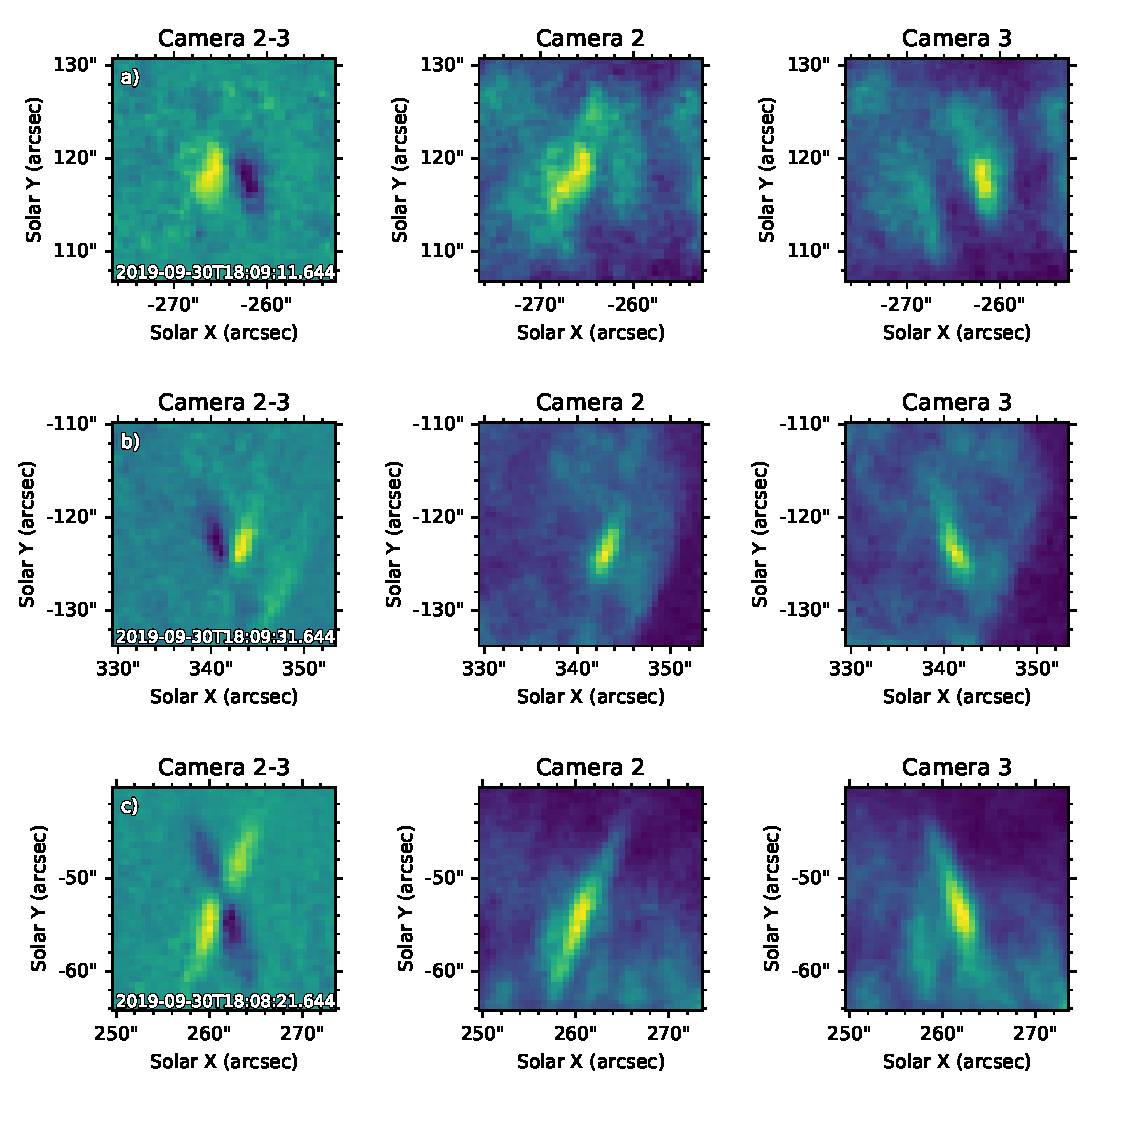
\includegraphics{dif_events}
   			\caption{\jdp{Update}Events a, b and c identified in Figure \ref{fig:l3_dif} are examples of a mostly blue, red, and broadened even, respectively. The difference between Channels 2 and 3 is shown in the left hand column, while the Channel 2 and Channel 3 intensities are shown in the middle and right columns.  The velocity signature is most easily seen in the difference image, while the straight intensities provide information on the line core intensities. 
   			}
   			\label{fig:dif_events}. 
   		\end{figure}

    	Simple, point-like, transient brightenings with little or no spatial structure are the easiest events to interpret because their naturally confined spatial extent acts similarly to a spectrographic slit.
    	For that reason any stretching along the dispersion direction in an ESIS image can be interpreted directly as velocity. 
    	In these simple events, a qualitative understanding of their velocity can be ``read off'' of each ESIS difference image.
    	This effect was explored in great detail by \citet{Rust2019}, who sliced through small events along the dispersion direction to measure \heii \ line profiles from MOSES data.
    	
    	Here we explore the velocity signature in three examples of simple point-line events marked a-c in Figure~\ref{fig:l3_dif}.  
    	Figure \ref{fig:dif_events} shows the difference image in the first column for all three events, then the Channels 2 and 3 data in the subsequent columns. 
    	Figure \ref{fig:dif_events}a shows a V-shaped event that is pointed downward in the difference between the Channel 2 and Channel 3 Level-3 image.
    	Since we know that the direction of positive wavelength dispersion is up and to the right in Channel 2 and up and to the left in Channel 3 (Figure \ref{fig:mgx_overlap}) we immediately know that this event is predominantly blue shifted.  
    	Similarly, an upward facing V-shaped event, like the one shown in Figure \ref{fig:dif_events}b, is predominantly red shifted.
    	X-shaped events, shown in Figure \ref{fig:dif_events}c, that occur equally if not more frequently than V-shaped events, suggest enhanced emission in both the red and blue wing of the line profile.
    	Difference images can provide immediate qualitative understanding of these simple, point-like events.  
    	During the 5 minute rocket flight, tens of similar events were detected in the ESIS field of view.  
    	
    	%While this gives us a quick and qualitative understanding of a simple event, even the smallest amount of spatial extent in a given feature leads to an entanglement of spatial and spectral information making it very difficult to derive qualitative velocities without inversion. 
    	
    	\begin{figure}[htb!]
    		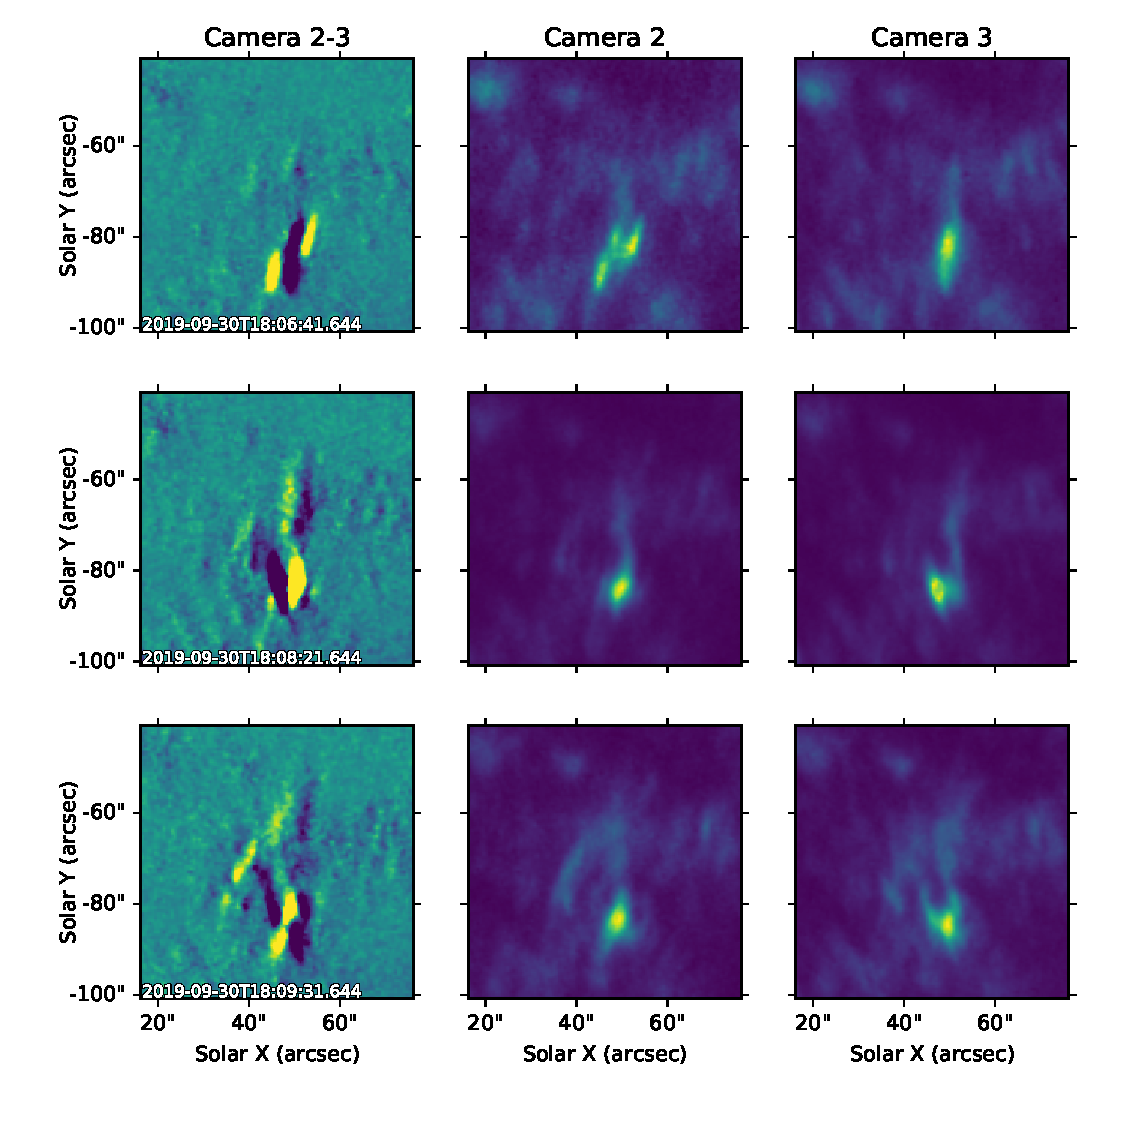
\includegraphics{main_event}
    		\centering
    		\caption{\jdp{update.  Also, it might be sweet to animate this one for the paper.} The largest eruption captured by ESIS shown at three different times. The event starts with as two jets (one red, one blue) with slight spatial separation, evolves into a strong red shift where the event begins paired with faint blue shifted material above, and ends in a complicated combination of velocity not easily interpreted from difference images. }
    		\label{fig:main_event}
    	\end{figure}
		
    	During the ESIS flight, we also captured a handful spatially extended objects that are more difficult to interpret.
    	The most obvious of these is an eruption near disk center, Event e in Figure \ref{fig:l3_dif}.
    	This large event is shown at three times in Figure \ref{fig:main_event}.
    	As shown, an erupting two-dimensional feature leads to an entanglement of spatial and spectral information that makes it very difficult to derive qualitative velocities without inversion.
    	In difference images (left column) there is a mess of positive and negative features intertwined in the brightest portion of the event that sometimes present as a V or X shape, but not always, and evolve significantly in time.
    	The top row shows this event early in it's evolution. 
    	Intensity is concentrated to a small region and presents as two jets, one red and one blue, with a slight spatial separation.
    	Shortly after (middle row) the event is dominated by a significant red shift (upward facing V) at the location of initial brightening, 
    	There is also an imprint of fainter differences above the brightest knot of intensity showing motion along a spatially extended structure.
    	The difference in this faint structure is opposite in polarity to the intensity below, and therefore appears to be ejected blue shifted material from the site of initial brightening.
    	By the end of the event (bottom row), the dominate red shift subsides, leaving a complicated spectral signature and the brightest portion of the event, and in adjacent region up and to the left.  
    	Dynamic and spatially extended events are excellent opportunities for ESIS to shine and clearly demonstrate the need for many different projection angles (ESIS channels) if we hope to disentangle spatial information from spectra.
    	Despite the extra complexity, an understanding of ESIS difference images provides an excellent sanity check when interpreting future inversions.
    	In the following section we will focus on inverting two smaller events (c and d), and will save a more in depth analysis of Event E for a future publication. 
    	
    
    % 	Larger positive or negative features with no obvious counterpart nearby, are indicative of spectral contamination \citep{RustPhD,Parker2021}.
    % 	The most easily seen impact of this is a faint octagon edge visible in Figure \ref{fig:l3_dif} from Mg {\sc x} 625.9 \AA.
    % 	Extra spectral content will act as a source of error when inverting Level-3 data, but will be properly accounted for by a wavelength dependent optical distortion model and the completion of the ESIS Level-2 data set \citep{Smart2022}. 	 
    % 	\amy{roy's paper already slated for 2022?  I mention some of this above, don't know if we need to keep it in both places.}
    
    
    \subsection{Early Inversions} \label{sec:inversions}
    	In order to better disentangle the spectral and spatial information captured by ESIS, information from every channel is combined and ``inverted'' to return a single, spatial-spectral cube, at every exposure.
    	For out preliminary inversions of ESIS Level-3 data we used a Multiplicative Algebraic Reconstruction Technique (MART).
    	MART is attractive for our first inversions because it is fast, requires no training or assumptions about the data, and automatically enforces image  positivity.
    	We describe our particular implementation in more detail in Appendix \ref{MART}.
    	
    	\begin{figure}[htb!]
    		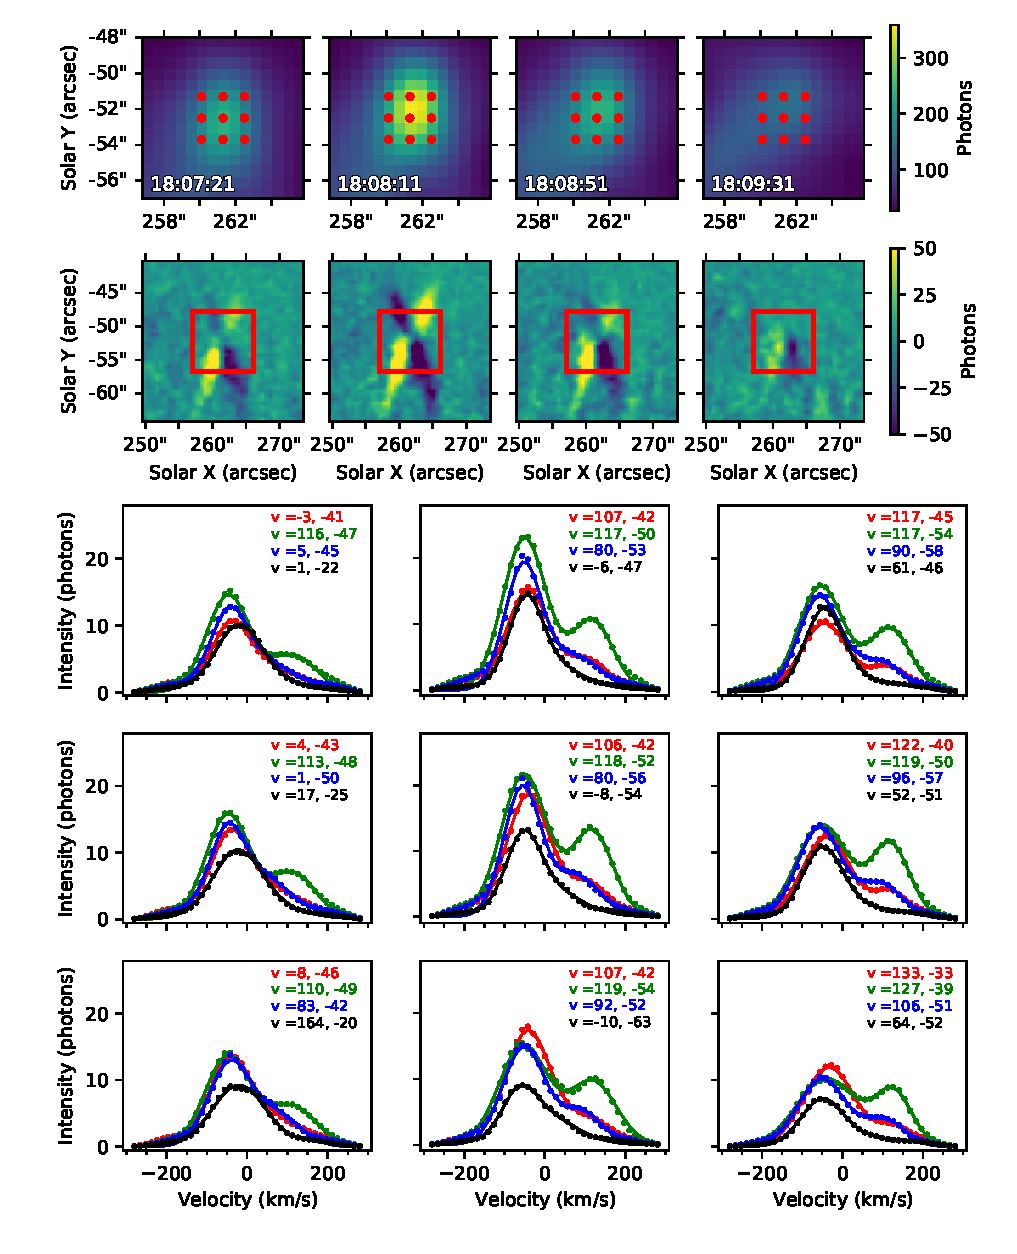
\includegraphics{perfect_x_inverted}
    		\centering
    		\caption{MART inverted results of event c in Figure \ref{fig:l3_dif}. The integrated intensity (top row) and corresponding Level-3 difference image (second row) are shown at 4 different times. A red box on each difference image marks the FOV used in the top row.  The \ov \ line profile at each position marked with a red dot is plotted in the matching 3x3 grid in a different color for each time (in order red, green, blue, black). Each MART line profile (dots) is overplotted with a double gaussian fit (solid line).  Bulk shifts in km/s for each component of the fit are added for each time in their respective color. }
    		\label{fig:perfect_x_inverted}
    	\end{figure}
        
        \begin{figure}[htb!]
    	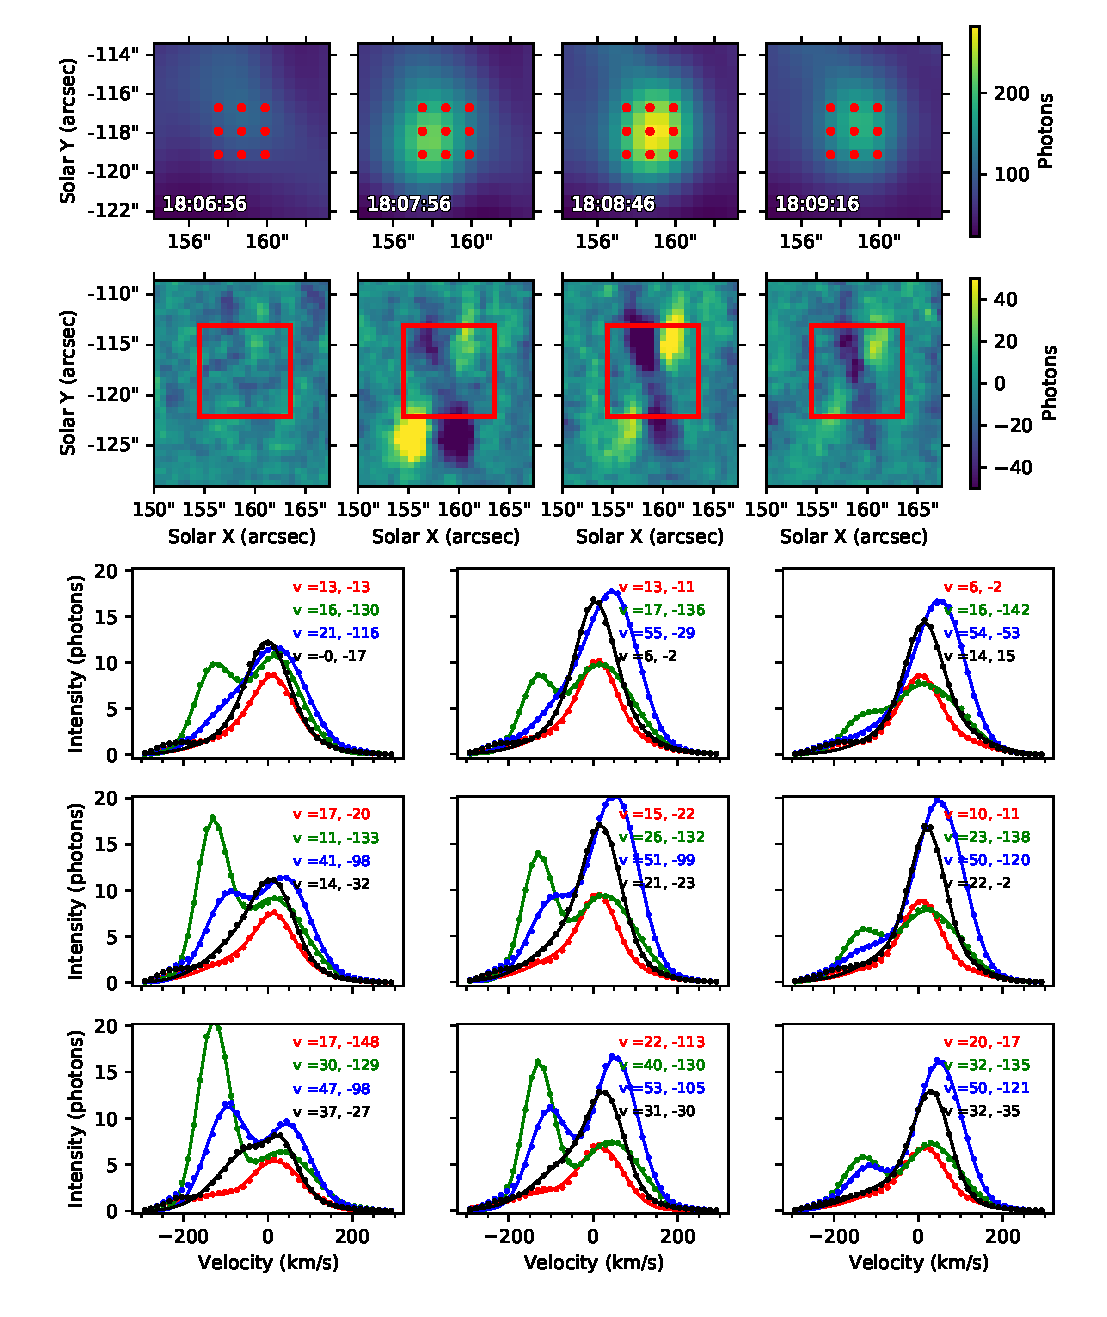
\includegraphics{other_x_inverted}
    	\centering
    	\caption{MART inverted results for event d in Figure \ref{fig:l3_dif} presented in the same fashion as Figure \ref{fig:perfect_x_inverted}.}
    	\label{fig:other_x_inverted}
    	\end{figure}
    	
    	In Figures \ref{fig:perfect_x_inverted} and \ref{fig:other_x_inverted}, and their associated animations, we present the MART inversion for two different compact transient events, labeled c and d in Figure \ref{fig:l3_dif}.
    	Both events have an X-shaped presentation, begin and end within the ESIS observing time, and show noticeable temporal evolution in velocity.
		Each figure shows the total integrated intensity (top row) and Channel 2-3 Level-3 difference image (second row) at four different times.  
		The FOV of the integrated intensity is shown as a red box on the difference image below. 
		Inverted \ov \ line profiles at each spatial location marked by a red dot in the integrated intensity image are plotted in the matching 3x3 grid for each time (in the order red, green, blue, black).
		We performed a double gaussian fit for each line profile in order to more easily pick out the location of each peak in velocity.
		The results of the fit (solid line) is plotted over the MART inverted data (dots).
		The deviation from line center of each gaussian is recorded in km s$^{-1}$ in the color matching line profile.
		In the animation, we plot the red and blue components of each fit separately as dashed lines, their sum as a solid line in fuschia, and the MART inverted line profile in  green dots.
		
		Event c described Figure \ref{fig:perfect_x_inverted} lasts just over 4 minutes and shows significant temporal evolution in the line profile.
		Throughout the event the blue component of the \ov \ line dominates and is centered at $\approx$ -50 km s$^{-1}$.
		This blue component persists for the entire duration of the event with very slight deviations intensity and velocity.
		The red component of the event is bursty in nature, with two small peaks in intensity at 18:07:41 and 18:08:11, and is centered at $\approx$ 110 km s$^{-1}$.
		While there are a several frames where the red component of the line appears as an additional peak in the line profile and is well fit by a second gaussian, most of the time it presents more as an asymmetric broadening in the red wing of the line making the velocities from the fit less reliable.
		This explosive event is $\approx$ 3 arcseconds in diameter and shows little spatial variation in the line profile across the event.
		
		The explosive event highlighted Figure \ref{fig:other_x_inverted}, event d, is similar to event c in that is has enhancements in both the red and blue wing of the line profile, but is more complicated in it's presentation.
		Event d  begins at 18:07:11 and it's intensity has almost completely died away by the last Level-3 image, but not entirely. 
		\jdp{verify time after Level-3 rebuild}
		A strong blue component in the line profile centered near -125\,km\,s$^{-1}$  peaks at 18:08:01 dominates early in the event evolution.
		This blue component is brightest in the lower left portion of the event.
		The red component of the line profile peaks at 18:08:51 and is centered near 50 km s$^{-1}$.
		Unlike event c, the blue component of the line is less persistent in time.
		Also, the blue and red components of the event do not occur in the same spatial location.
		This is visible both in the grid of line profiles and the difference images.
		Intensity in the line profiles show the blue component peaking in the lower left, while the red component peaks in the middle to right columns.
		In the difference images there is a clear vertical and horizontal separation between the blue downward facing V and the red upward facing V. 
		A closer look at the inverted data shows an $\approx$ 1.35 arcsecond spatial separation between centroids of the blue and red component.

		Despite a couple free parameters in our MART algorithm, namely the exponent used on the contrast enhancement filter and the number of times it is applied (Appendix \ref{MART} steps \ref{step:contrast} and \ref{step:smooth}) we consistently find line profiles consistent with a qualitative interpretation of the difference image movies, and measure bulk flows within $\approx\pm$ 15\,km\,s$^{-1}$ of each other for a given exposure.
		Figure \ref{fig:perfect_x_invert} shows the results of tweaking these free parameters for a single timestamp of Event C and is paired with an explanation of their impact in Appendix \ref{MART}.
	    		   	
    	
\section{Discussion/Conclusions and Future Work}
	The ESIS sounding rocket mission, launched September 30th 2019, was successful in capturing spatial and spectral information over is entire \esisfov \ field of view in multiple wavelengths (\hei, \mgxbright, and \ov) at every exposure.
	We have processed the data into multiple levels such that preliminary scientific work can be done, included a Level-3 data product that allows for taking spatial differences between channels, and early inversion (Section \ref{sec:level-3}).
	Level-3 difference images in the \ov \ wavelength (Section \ref{sec:dif_images}) reveal a host of small transient brightenings across the field of view with significant line-of-sight Doppler velocity, some in excess of $\pm 100\,$km\,s$^{-1}$.
	They also real several larger events with large velocities, most notably the eruption identified near disk center (event e in Figure \ref{fig:l3_dif}).
	
    During the roughly 5 minutes of ESIS observing time it captured tens of events, evolving on 10 seconds timescales, over it's 11.3\,arcminute field of view.
	Even seemingly simple explosive events evolve fast enough in time, and have significant spatial distributions of intensity and velocity, such that rastering a traditional slit spectrograph would fail to capture the event completely. 
	This combined with the fact that ESIS can measure tens of events like this simultaniously makes it a powerful tool for capturing and diagnosing small eruptions in the solar atmosphere.
	
	We use a Multiplicative Algebraic Reconstruction Technique (MART, Appendix \ref{MART}) to disentangle the combined spatial and spectral information in the four ESIS Level-3 images to find a single spatial-spectral cube ([x,y,$\lambda$]), covering just the  \spectralline{O}{v}{630} line, for two small transient brightenings (Section \ref{sec:inversions}).
	Our inversions reveal strong red and blue jets with bulk flows in excess of 100\,km s$^{-1}$ that evolve on the timescale of the ESIS cadence, 10 seconds.
	These two events are spatially compact, a few arcseconds, and have lifetimes of a few minutes.
	Despite their compact nature, the red and blue components measured are separate and distinct in both space and time. 
	This is especially noticeable in event d (Figure \ref{fig:l3_dif} and \ref{fig:other_x_inverted}) where the centroids of the blue and red jet are displaced by a little over an arcsecond. 
	
	The bimodal nature and absence of line core emission in these small brightenings is similar observations made by \citet{Rust2019} \heii \ using MOSES data.
	This presentation is quite different from line profiles observed by IRIS \citep{depontieu2014} in \spectralline{Si}{iv}{1394}, where small transient events show smaller bulk flows, dominant line core emission, and excessive non-thermal broadening.
	Assuming such high bulk flows are indicative of reconnection outflows, suggests a very small reconnection region with little to no stationary emitting plasma, pointing away from a dominate tearing mode instability, and toward a Petschek type reconnection.
	Though we hypothesize that both jets originate at a single reconnection site, we admit that it is puzzling that observed fluctuations of the red and blue jets are not temporally correlated, most noteably in explosive event d (Figure \ref{fig:other_x_inverted}). 
	It may be that the reconnection in these small events is more complex than we imagine; however, it is also possible that, looking in a single spectral line, we are not seeing all of the ejected plasma. 
	Further work with the ESIS data may help to clarify this issue.
	Several of these events were captured in \hei, \mgxbright, and \ov \ simultaneously, putting ESIS in a position to measure the outflows at multiple temperatures. 
	We can also see if the bi-modal nature of these line profiles is unique to \ov \ or persists at lower and higher temperatures.
	Also, IRIS was running small four step coarse rasters near disk center during the hour long ESIS launch window.
	Although none of the events analyzed in this paper were captured by IRIS, a closer look at the IRIS data may reveal small explosive events suitable for direct comparison with ESIS line profiles.
	
	The next major tasks in the analysis of ESIS data will be to invert the entire spatial-spectral cube, from \spectralline{He}{ii}{584} to \spectralline{O}{v}{630}. 
	A self-consistent inversion will be required to separate out the dimmer \mgxdim, and perhaps even the faint \oiii \ line. This will require a careful characterization of the wavelength-dependent distortion in the images, which is currently underway.
	Future multi-wavelength inversions of the ESIS data will allow for more accurate estimates of the frequency and distribution of explosive events across a large portion of the solar disk and at different heights in the solar atmosphere than have been possible with slit spectrographs.
	It will also allow us to track energy and material moving through multiple layers of the solar atmosphere to form a clearer picture of where and how these reconnection events unfold. 
	
	\jdp{Do we need one more paragraph where we compare Event E to a mini filament eruption and cite a few papers?  Also, should we mention coordinated data from the mission (i.e. SOT/ESIS/IRIS ?)}
	

\begin{acknowledgements}
	\jdp{ESIS grant number?}
	CHIANTI is a collaborative project involving George Mason University, the University of Michigan (USA), University of Cambridge (UK) and NASA Goddard Space Flight Center (USA).
	This research used version 0.5.0 (10.5281/zenodo.4676478) of the aiapy open source software package \citep{aiapy}.
	
	
\end{acknowledgements}



\appendix
\section{Multiplicative Algebraic Reconstruction Technique}\label{MART}
	Multiplicative Algebraic Reconstruction Technique (MART) has been applied to limited-angle tomography problems that are very similar to the ESIS data reconstruction problem \citep{Okamoto1991,Verhoeven1993}.
	When testing a variety of inversion methods on MOSES data \citet{FoxPhD} identified MART as most promising of several methods in terms of speed and fidelity.
	\citet{RustPhD} applied a slightly different version of MART to the MOSES data paired with a wavelet based partial reconstruction technique for better background subtraction and event isolation.
	Due to it's speed, lack of required training, and automatic enforcement of image positivity we have chose MART for our first inversion of Level-3 ESIS data.
	
	With MART we seek to reconstruct the true spatial-spectral cube, $I_{xy\lambda}$, using every ESIS image or projection, $f_{\theta x'y'}$. There is one ESIS image for each $\theta$ representing the relative orientations of each ESIS channel. The procedure is executed as follows:
	\begin{enumerate}
		\item \label{step:guess} Create a guess cube, $G_{xy\lambda} = 1$ on the same domain as $I$. 
		\item \label{step:contrast} Enhance the contrast of $G$ and normalize. 
			\begin{equation}
				G \leftarrow \frac{G+G^{(1+\Psi)}}{\sum_{xy\lambda}G+G^{(1+\Psi)}}\sum_{xy\lambda}G, 
			\end{equation}
		
		\item \label{step:smooth} Convolve $G$ with smoothing kernel $K$, $G \leftarrow G * K$,
		in our case,
			\begin{equation}
			\label{eq:kernel}
				K_{ijk} = \frac{2^{3-|i|-|j|-|k|}}{64} \quad \text{for}\quad i,j,k = -1,0,1.
			\end{equation}
		
		\item \label{step:project} Sum $G_{\theta xy\lambda}$ along lines of constant $x-\delta\lambda$ to calculate a projection for each angle $\theta$,
			\begin{equation}
				f'_{\theta x'y'} = \sum_\lambda G_{\theta(x-\delta\lambda)y\lambda}, 
			\end{equation}
		where,
			\begin{equation}
				G_{\theta xy\lambda} = \mathcal{R}_\lambda(\theta)\,G_{xy\lambda},
			\end{equation} 
		and, $\mathcal{R}(\theta)$, is a rotation about the $\lambda$ axis. 	
		
		\item \label{step:chisquared} Calculate reduced chi-squared for each projection and check for convergence, in this case that $\chi_{R,\theta}^2 < 1$ , 
			\begin{equation}
				\chi_{R,\theta}^2 = \frac{1}{N_{x'} N_{y'}}\sum_{x'y'} \frac{(f_{\theta x'y'}-f'_{\theta x'y'})^2}{f'_{\theta x'y'}+\sigma^2_{RN}},
			\end{equation}
		where $\sigma^2_{RN}$ is the read noise in photons squared, $N_{x'}$ is the total number of elements along $x'$.
		
		\item Calculate correction factors for each unconverged channel, $\theta_{uc}$, weighted by $\gamma$, 
			\begin{equation} \label{eq:correctionfactor}
				c_{\theta x'y'} = \left[\frac{f'_{\theta x'y'}}{f_{\theta x'y'}}\right]^\gamma,
			\end{equation}
		where $\gamma = 2/n$ with $n$ equal to the total number of channels.
		
		\item Assign correction factors to lines of constant $x-\delta\lambda$ in the domain of $G$,
			\begin{equation}
				C_{\theta (x-\delta\lambda)y\lambda} = c_{\theta x'y'}
			\end{equation}	
		
		\item \label{step:correct} Apply a weighted product to each derotated correction to $G$ ,
			\begin{equation}\label{eq:correct}
				G \leftarrow G\left\lbrace  \,\prod_{\theta=\theta_{uc}}  \mathcal{R}_\lambda(-\theta_i)C_{\theta xy\lambda} \right\rbrace^{1/m_{uc}},
			\end{equation}
		where $m_{uc}$ is the total number of unconverged channels and 
		
		\item Repeat steps \ref{MART}\ref{step:project}-\ref{MART}\ref{step:correct}
		until every channel has converged at step \ref{MART}\ref{step:chisquared}.
	\end{enumerate}
		For this particular implementation we use a contrast enhancement exponent of $\Psi = .2$ and have a total number of channels, $n=4$.
		The spectral dispersion of an ESIS grating, $\delta$ is equal to 28 m\AA\ pix$^{-1}$. 
		We construct $G$ such that its resolution in $\lambda$ is equal to $\delta$.
		All negative values introduced by rotation (from ringing near the data edge) are set to zero after each rotation.
		
		\begin{figure}[htb!]
			\begin{tikzpicture}
			
			%begin by adding a node for each figure
			\node[inner sep=0pt] (imgs) at (0,0)
			{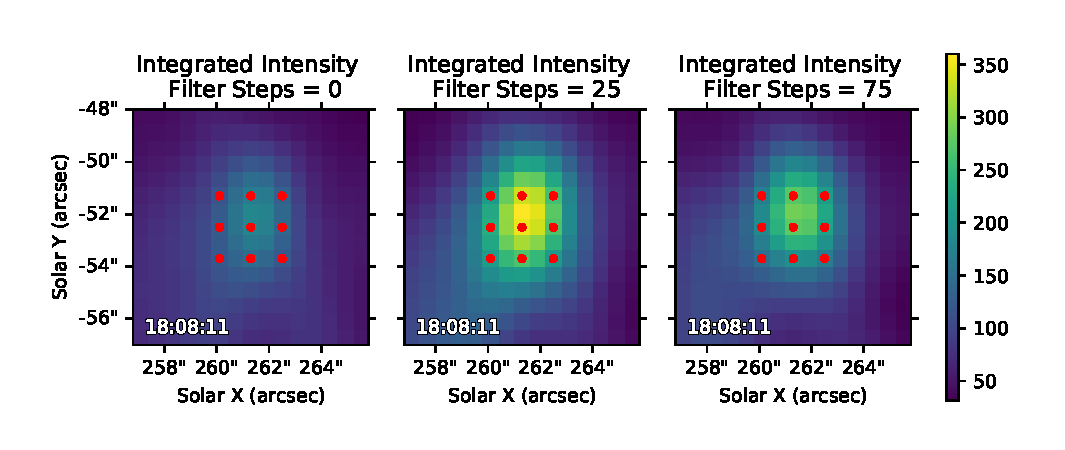
\includegraphics[]{perfectx_invert_comp_a}};
			\node[inner sep=0pt] (lps) at (0,-9.5)
			{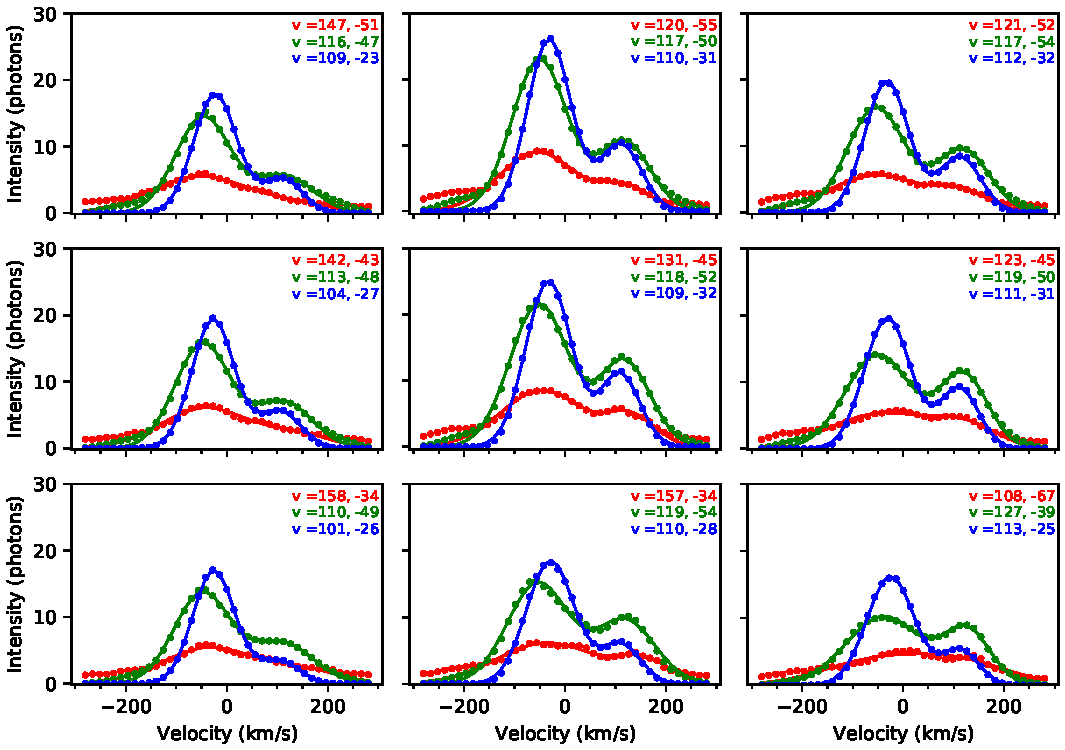
\includegraphics[]{perfectx_invert_comp_b}};
			
			
			\end{tikzpicture}
			\centering
			\caption{Comparison of MART ouputs for a single timestamp in Event c (Figure \ref{fig:l3_dif} and \ref{fig:perfect_x_inverted}).}
			\label{fig:perfect_x_invertcomp}
		\end{figure}
		
		
		The contrast enhancement and smoothing step are designed to fight the tendency of MART to smear intensity along the dispersion directions in a way that matches the data, but results in artificial intensity way in the wings of the inverted spectra (referred to as ``plaid'').
		Each time the filter is applied (steps \ref{MART}\ref{step:contrast} and \ref{MART}\ref{step:smooth}) steps \ref{MART}\ref{step:project}-\ref{MART}\ref{step:correct} are repeated until convergence in every channel.
		
		

		
		
		The impact of plaid is most evident in the red spectral lines in Figure \ref{fig:perfect_x_invertcomp} where the contrast enhancement filter wasn't used at all.
		Despite excess intensity in the wings of the lines, the brightest pixels are still double peaked in nature and the two Gaussian fits do a decent job of fitting the inverted line profiles.
		The blue spectral lines in Figure \ref{fig:perfect_x_invertcomp} show line profiles after repeating the contrast enhancement step enough times such that the solution reaches an equilibrium and returns the same results once converged.
		Since the contrast enhancement filter is designed to pull intensity from the background and into regions of stronger signal, it has the effect of clumping the intensity into a smaller area.
		This causes much less intensity in the wings of the line profile and narrower peaks overall.  
		Unfortunately this also has the ill effect of clumping background intensity where there is little signal instead of allowing for a flat noisy background as expected.  
		Therefore we choose to compromise and run the filtering step enough times such that the majority of the artificial intensity in the wings has been beaten down, but not so much that we artificially remove a flat noisy background in low signal regions.  
		To do this we landed on running the filtering step 25 times, and using a contrast enhancement exponent of .2 in an effort to not over filter the MART results.
		  

